\chapter{Integration}

\section{Reimann Integral over a Rectangle}

\begin{definition}
    Consider a rectangle $Q=[a_1,b_1]\times [a_2,b_2]\times \cdots \times[a_n,b_n]\subset \R^n$.
    \begin{itemize}
        \item Each of the interval $[a_i,b_i]$ is called a \underline{component interval} of $Q$.
        \item $\max\{b_1-a_1,b_2-a_2,\cdots ,b_n-a_n\}$ is called the \underline{width} of $Q$.
        \item $v(Q)=(b_1-a_1)\times(b_2-a_2)\times \cdots \times(b_n-a_n)$ is called the \underline{volume} of $Q$.
    \end{itemize}
\end{definition}
\noindent \textbf{Remark}:
\begin{itemize}
    \item In the case $n = 1$, the volume and the width of the (1-dimensional)
    rectangle $[a, b]$ are the same, namely, the number $b-a$. This number is also called the \underline{length} of $[a, b]$.    
\end{itemize}

\begin{definition}
    Given a closed interval $[a, b]$ of $\R$, a \underline{partition} of $[a, b]$ is a finite collection $P$ of points of $[a, b]$ that includes the points $a$ and $b$.
    $$P=\{a=t_0,t_1\cdots,t_{k-1},t_k=b\}$$
    where $t_i$ are in increasing order for convenience. Each interval $[t_{i-1},t_i]$ is called a \underline{subinterval} determined by $P$ of the interval $[a,b]$.
\end{definition}

\begin{definition}
    Let $Q=[a_1,b_1]\times [a_2,b_2]\times \cdots \times[a_n,b_n]\subset \R^n$. A \underline{partition} $P$ of $Q$ is an n-tuple $$P=(P_1,P_2,\cdots,P_n)$$ where each $P_i$ is a partition of $[a_i,b_i]$ for each $i$. 
    If for each $i$, $I^{(i)}_j$ is one of the subintervals determined by $P_i$ of the interval $[a_i,b_i]$, then the rectangle $$R=I^{(1)}_{j_1}\times I^{(2)}_{j_2}\times \cdots \times I^{(n)}_{j_n}$$ is called a \underline{subrectangle} determined by $P$, of the rectangle $Q$. 
    The maximum width of these subrectangles is called the \underline{mesh} of $P$.
\end{definition}

\begin{definition}
    Let $Q\subset \R^n$ be a rectangle and let $f:Q\longrightarrow \R$. Assume $f$ is bounded. Let $P$ be a partition of $Q$. For each subrectangle $R$ determined by $P$, define
    $$m_R(f)=\inf\{f(x): x\in R\}$$
    $$M_R(f)=\sup\{f(x): x\in R\}$$
\end{definition}

\begin{definition}
    Similar to single variable calculus, we can define the \underline{lower sum} and the \underline{upper sum} respectively of $f$ determined by $P$,
    $$L(f,P)=\sum_Rm_R(f)\cdot v(R)$$
    $$U(f,P)=\sum_RM_R(f)\cdot v(R)$$
    where the summations extend over all subrectangles $R$ determined by $P$.
\end{definition}

\begin{definition}
    Let $P=(P_1,P_2,\cdots,P_n)$ and $P'=(P_1',P_2',\cdots,P_n')$ be partitions of $Q$.
    \begin{itemize}
        \item If $P_i \subset P_i'$ for all $i$, then $P'$ is called a \underline{refinement} of $P$.
        \item Can also define a new partition based on $P$ and $P'$,
        $$P''=(P_1 \cup P_1',P_2\cup P_2',\cdots,P_n\cup P_n')$$
        $P''$ is called the \underline{common refinement} of $P$ and $P'$.
    \end{itemize}
\end{definition}

\begin{lemma}
    Let $P=(P_1,P_2,\cdots,P_n)$ and $P'=(P_1',P_2',\cdots,P_n')$ be partitions of $Q\subset \R^n$ and $P'$ refines $P$. Let $f:Q\longrightarrow \R$. Then we have
    $$L(f,P)\leq L(f,P') \text{ and }U(f,P')\leq U(f,P)$$
\end{lemma}


\begin{lemma}
    Let $Q$ be a rectangle; let $f:Q\longrightarrow R$ be a bounded function. If $P$ and $P'$ are any two partitions of $Q$, then
    $$L(f,P)\leq U(f,P')$$
\end{lemma}


\begin{theorem}
    Let $P=(P_1,P_2,\cdots,P_n)$ and $P'=(P_1',P_2',\cdots,P_n')$ be partitions of $Q\subset \R^n$ and $P'$ refines $P$. Let $f:Q\longrightarrow \R$. Then we have
    $$L(f,P)\leq L(f,P') \leq U(f,P')\leq U(f,P)$$
\end{theorem}

\begin{definition}
    Let $Q\subset \R^n$ be a rectangle. Let $f:Q\longrightarrow \R$ be a bounded function. Let $\mathcal{P}$ denotes the set of all partitions of $Q$.
    \begin{itemize}
        \item \underline{Lower integral}: $$\underline{\int_Q}f=\sup\{L(f,P):P\in\mathcal{P}\}$$
        \item \underline{Upper integral}: $$\overline{\int_Q}f=\inf\{U(f,P):P\in\mathcal{P}\}$$
    \end{itemize}
\end{definition}

\begin{definition}
    We say $f$ is \underline{integrable} over $Q$ if the upper and lower integrals of $f$ over $Q$ are equal.
    We denote the integral as $$\int_Qf\text{ or }\int_{x\in Q}f(x)$$
\end{definition}
\noindent \textbf{Remark}:
\begin{itemize}
    \item The lower integral represents the so-called “inner area” of this region, computed by approximating the region by inscribed rectangles, while the upper integral represents the so-called “outer area,” computed by approximating the region by circumscribed rectangles. If the “inner” and “outer” areas are equal, then $f$ is integrable.
\end{itemize}
\noindent \textbf{Example}:
\begin{itemize}
    \item If Q is a rectangle in $\R^2$ and $f: Q \longrightarrow \R$ is non-negative and bounded, one can picture $L(f,P)$ as the total volume of a bunch of boxes inscribed in the region between the graph of $f$ and the xy-plane, and $U(f, P)$ as the total volume of a bunch of boxes circumscribed about this region.
    \begin{figure}[ht]
        \centering
        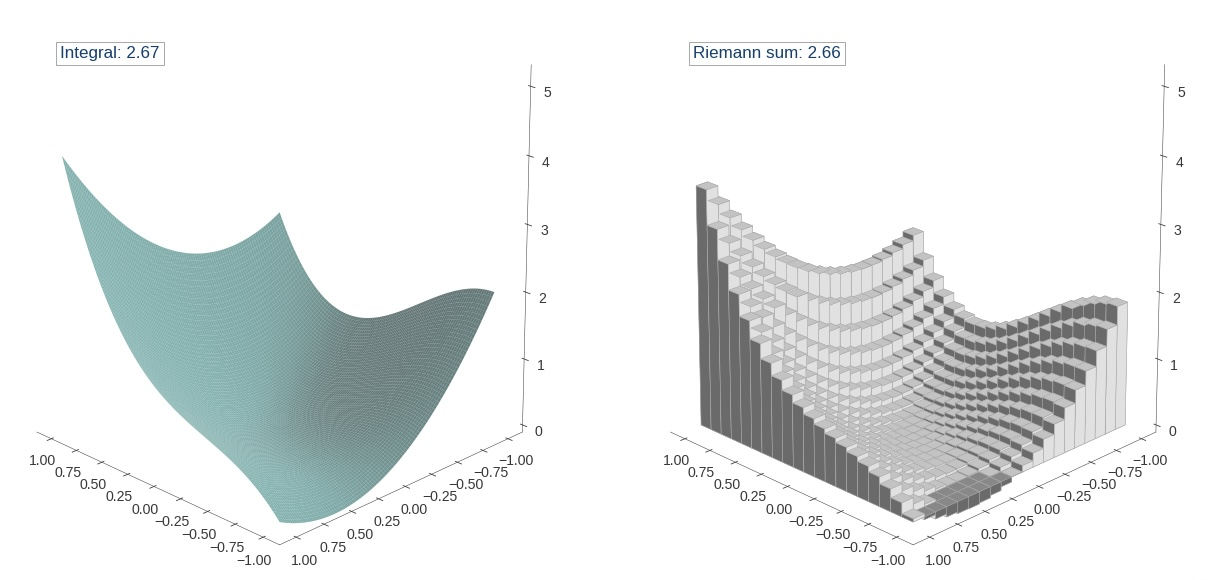
\includegraphics[scale=0.32]{images/fig4031-riemann-integration-multivariate.jpeg}
        \caption{Picture of Reimann sum}
    \end{figure}
\end{itemize}

\begin{theorem}[The Riemann Condition]\label{The Riemann Condition}
    Let $Q\subset \R^n$ be a rectangle, let $f:Q \longrightarrow \R$ be bounded. Let $\mathcal{P}$ be the set of all partitions of $Q$. Then $f$ is integrable if and only if 
    $$\forall \epsilon >0. \exists P \in \mathcal{P}. U(f,P)-L(f,P)<\epsilon$$
\end{theorem}

\begin{theorem}\label{sum of subrectangles}
    Let $Q\subset \R^n$ be a rectangle. Let $\{Q_1,\cdots,Q_k\}$ be a finite collection of rectangles that covers $Q$. Then 
    $$v(Q)\leq \sum_{i=1}^kv(Q_i)$$
\end{theorem}

\begin{theorem}\label{continuous implies integrable}
    Let $Q\subset \R^n$ be a rectangle, let $f:Q \longrightarrow \R$ be continuous. Then $f$ is integrable.
\end{theorem}

\section{Conditions for Integrability}

\begin{definition}
    We say $A\subset \R^n$ has \underline{measure zero} if for any $\epsilon>0$, there exists countably many rectangles $\{Q_1,Q_2,\cdots\}$ cover $A$ such that
    $$\sum_{i=1}^{\infty}v(Q_i)<\epsilon$$
    In this case, we say that the \underline{total volume} of the rectangles $Q_1,Q_2,\cdots$ is less than $\epsilon$.
\end{definition}

\begin{theorem}\ \label{measure zero 4 theorems}
    \begin{enumerate}
        \item If $B \subset A$ and $A$ has measure zero in $\R^n$, then so does $B$.
        \item All of $A_1,A_2,\cdots$ has measure zero in $\R^n$. Then $A=\bigcup_{i=1}A_i$ has measure zero in $\R^n$.
        \item A set $A$ has measure zero in $\R^n$ if and only if for every $\epsilon > 0$, there is a countable covering of $A$ by open rectangles $Int(Q_1), Int(Q_2),\cdots$ such that $$\sum_{i=1}^{\infty}v(Q_i)<\epsilon$$
        \item If $Q$ is a rectangle in $\R^n$, then $Bd(Q)$ has measure zero in $\R^n$ but $Q$ does not.
    \end{enumerate}
\end{theorem}

\noindent \textbf{Example}:
\begin{itemize}
    \item The \underline{cantor set} in $[0,1]$ is created by iteratively deleting the open middle third from a set of line segments
    \begin{itemize}
        \item $C_0:= [0,1]$
        \item $C_n:=\frac{C_{n-1}}{3}\cup (\frac{2}{3}+\frac{C_{n-1}}{3})$
    \end{itemize}
    So the formal definition of the cantor set is $$\mathcal{C}:=\lim_{n\to \infty}C_n=\bigcap_{n=1}^{\infty}C_n$$
    \begin{figure}[ht]
        \centering
        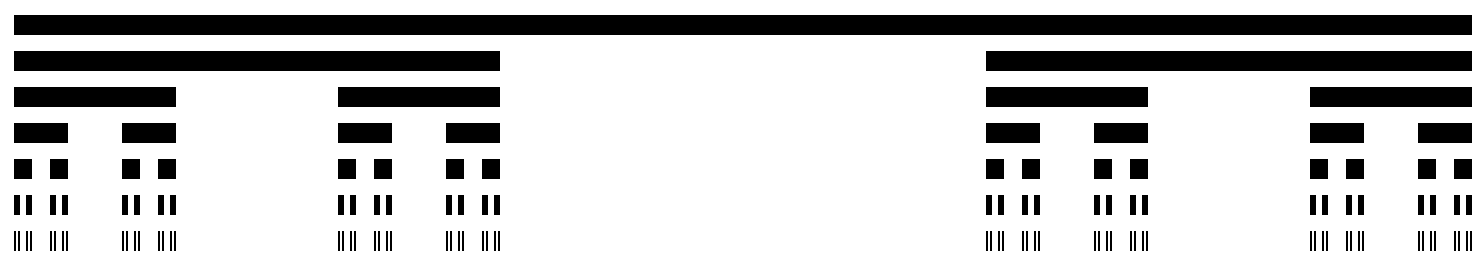
\includegraphics[scale=0.5]{images/cantor set.png}
        \caption{Picture of creating the cantor set}
    \end{figure}
    \underline{The fact is that the cantor set has measure zero.}
    \item Every k-dimensional subspace of $\R^n$ has measure zero if $k < n$. In other words, lines have no area, and planes have no volume. For example, the two dimensional sphere $\mathbb{S}^2$ has measure zero in $\R^3$.
\end{itemize}

\begin{definition}
    Let $Q$ be a rectangle in $\R^n$. Let $f:Q\longrightarrow \R$. $\forall a \in Q.\forall \delta>0$ let
    $$A_{\delta}=\{f(x): x\in Q \text{ and }x \in U(a;\delta)\}$$
    Also, we let
    $$M_{\delta}(f)=\sup A_{\delta}$$
    $$m_{\delta}(f)=\inf A_{\delta}$$
    Now we can define the \underline{oscillation} of $f$ at $a$ by the equation
    $$v(f;a):=\inf\{M_{\delta}(f)-m_{\delta}(f): \delta >0\}$$
    It is clear that $v(f;a)\geq 0$ always hold.
\end{definition}

\begin{lemma}
    $f$ is continuous at $a$ if and only if $v(f;a)=0$.
\end{lemma}


\begin{theorem} \label{bounded f integrable iff D measure zero}
    Let $Q$ be a rectangle in $\R^n$, let $f : Q \longrightarrow R$ be a bounded function. Let $D$ be the set of points of $Q$ at which $f$ fails to be continuous. Then $f$ is integrable if and only if $D$ has measure zero in $\R^n$.
\end{theorem}

\begin{theorem}
    Let $Q\subset \R^n$ be a rectangle. Let $f:Q\longrightarrow \R$. Assume $f$ is integrable on $Q$. Then
    \begin{enumerate}
        \item If $f$ vanishes except on a set of measure zero, then $\int_Qf=0$.
        \item If $f$ is non-negative and if $\int_Qf=0$, then $f$ vanishes except on a set of measure zero.
    \end{enumerate}
\end{theorem}

\section{Evaluation of Reimann Integral}

\begin{theorem}[Fundamental Theorem of Calculus]\label{FTC}\
    \begin{enumerate}
        \item If $f$ is continuous on $[a,b]$ and $F(x)=\int_a^xf(t)\di t$, then $$F'(x)=f(x)$$
        \item If $f$ is continuous on $[a,b]$ and $F$ is of class $C^2([a,b])$ such that $f(x)=F'(x)$, then $$\int_a^bf(x)\di x=F(b)-F(a)$$
    \end{enumerate}
\end{theorem}
\noindent \textbf{Remark}:
\begin{itemize}
    \item The part 1 of the theorem tells us the anti-derivative of $f$ always exists in theory.
    \item The part 2 of the theorem tells us we can claculate the integral of $f$ if we find the anti-derivative.
    \item The same difficulties of evaluating the integral occur with n-dimensional integrals.
    \item One way of approaching the problem is to attempt to reduce the computation of an n-dimensional integral to the presumably simpler problem of computing a sequence of lower-dimensional integrals.
\end{itemize}

\begin{theorem}[Fubini for continuous functions of two variable] \label{Fubini for continuous functions of two variable}
    Let $Q = [a, b] \times[c,d]\subset \R^2$ be a rectangle. Let $f:Q\longrightarrow \R$ be continuous, then the integral of $f$ over $Q$ is
    $$\int_Qf=\int_{y=c}^{y=d}\left(\int_{x=a}^{x=b}f(x,y)\di x\right)\di y=\int_{x=a}^{x=b}\left(\int_{y=c}^{y=d}f(x,y)\di y\right)\di x$$
\end{theorem}

\begin{figure}[ht]
    \centering
    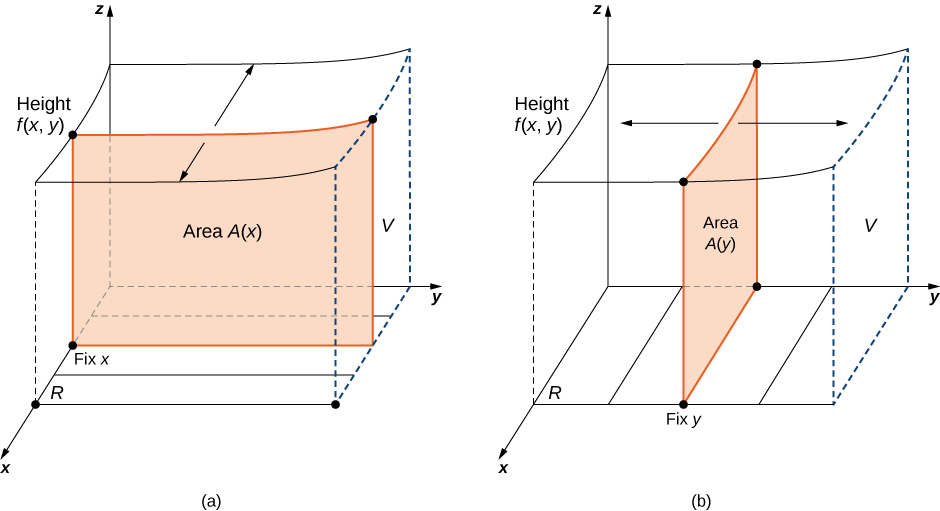
\includegraphics[scale=0.8]{images/CNX_Calc_Figure_15_01_006.jpg}
\end{figure}

\begin{theorem}[Fubini for continuous functions of n variable]
    Let $Q=[a_1,b_1]\times\cdots\times[a_n,b_n]\subset \R^n$ be a rectangle. Let $f:Q\longrightarrow \R$ be continuous. Then
    $$\int_Qf=\int_{x_1=a_1}^{x_1=b_1}\left[\int_{x_2=a_1}^{x_2=b_2}\left(\cdots\left(\int_{x_n=a_n}^{x_n=b_n}f(x_1,x_2,\cdots,x_n)\di x_n\right) \cdots \right)\di x_2\right]\di x_1$$
    and the order of the integration can be arbitrarily changed.
\end{theorem}

\noindent \textbf{Example}:
Let $Q=[0,\pi]\times[1,2]$, let $f(x,y)=sin(x)+y^2e^x$. Then
    \begin{equation}
        \begin{split}
            \int_Qf &= \int_{x=0}^{x=\pi}\left(\int_{y=1}^{y=2}(sin(x)+y^2e^x)dy\right)\di x\\
            &= \int_{x=0}^{x=\pi}\left(sin(x)y+\frac{y^3}{3}e^x\right)\Big|_1^2\di x\\
            &= \int_{x=0}^{x=\pi}\left(sin(x)+\frac{7}{3}e^x\right)\di x\\
            &= \left(-cos(x)+\frac{7}{3}e^x\right)\Big|_0^{\pi}\\
            &= \frac{7}{3}e^{\pi}-\frac{1}{3}
        \end{split}
    \end{equation}
\noindent \textbf{Remark}:
\begin{itemize}
    \item The theorems above are all about continuous functions. They are not usually proved in calculus. In fact, it is seldom mentioned that a proof is needed. They are taken as obvious. We can prove them with all the knowledge we have learnt.
    \item Our goal is to generalize these theorems to n-dimensional Euclidean space with integrable functions(may not be continuous). We will even generalize to metric space in the future. We should just prove the most generalized version(Fubini's Theorem).
    \item The following theorem is generalized from the theorem\ref{Fubini for continuous functions of two variable}. It is a corollary of the Fubini's Theorem.
\end{itemize}

\begin{theorem}
    Let $Q=I_1\times I_2\subset \R^2$ where $I_1,I_2$ are closed intervals in $\R$. Let $f:Q\longrightarrow\R$ be bounded. 
    If $\int_Qf$ exists, and if $\int_{y\in I_2}f(x,y)$ exists for each $x \in I_1$, then
    $$\int_Qf=\int_{x\in I_1}\int_{y\in I_2}f(x,y)$$
\end{theorem}

\noindent \textbf{Remark}:
\begin{itemize}
    \item It is possible for $f(x,y)$ to be integrable over $Q$, but $\int_{y\in I_2}f(x,y)$ does not exist for some $x$. Consider the following example: 
    Let $Q=[0,1]\times[0,1]$, define the function $f$ over $Q$
    \begin{equation}
        f(x,y)=
        \begin{cases}
            1\text{\quad if $x=0$ and $y$ is rational}\\
            0\text{\quad otherwise}
        \end{cases}
    \end{equation}
    \begin{figure}[ht]
        \centering
        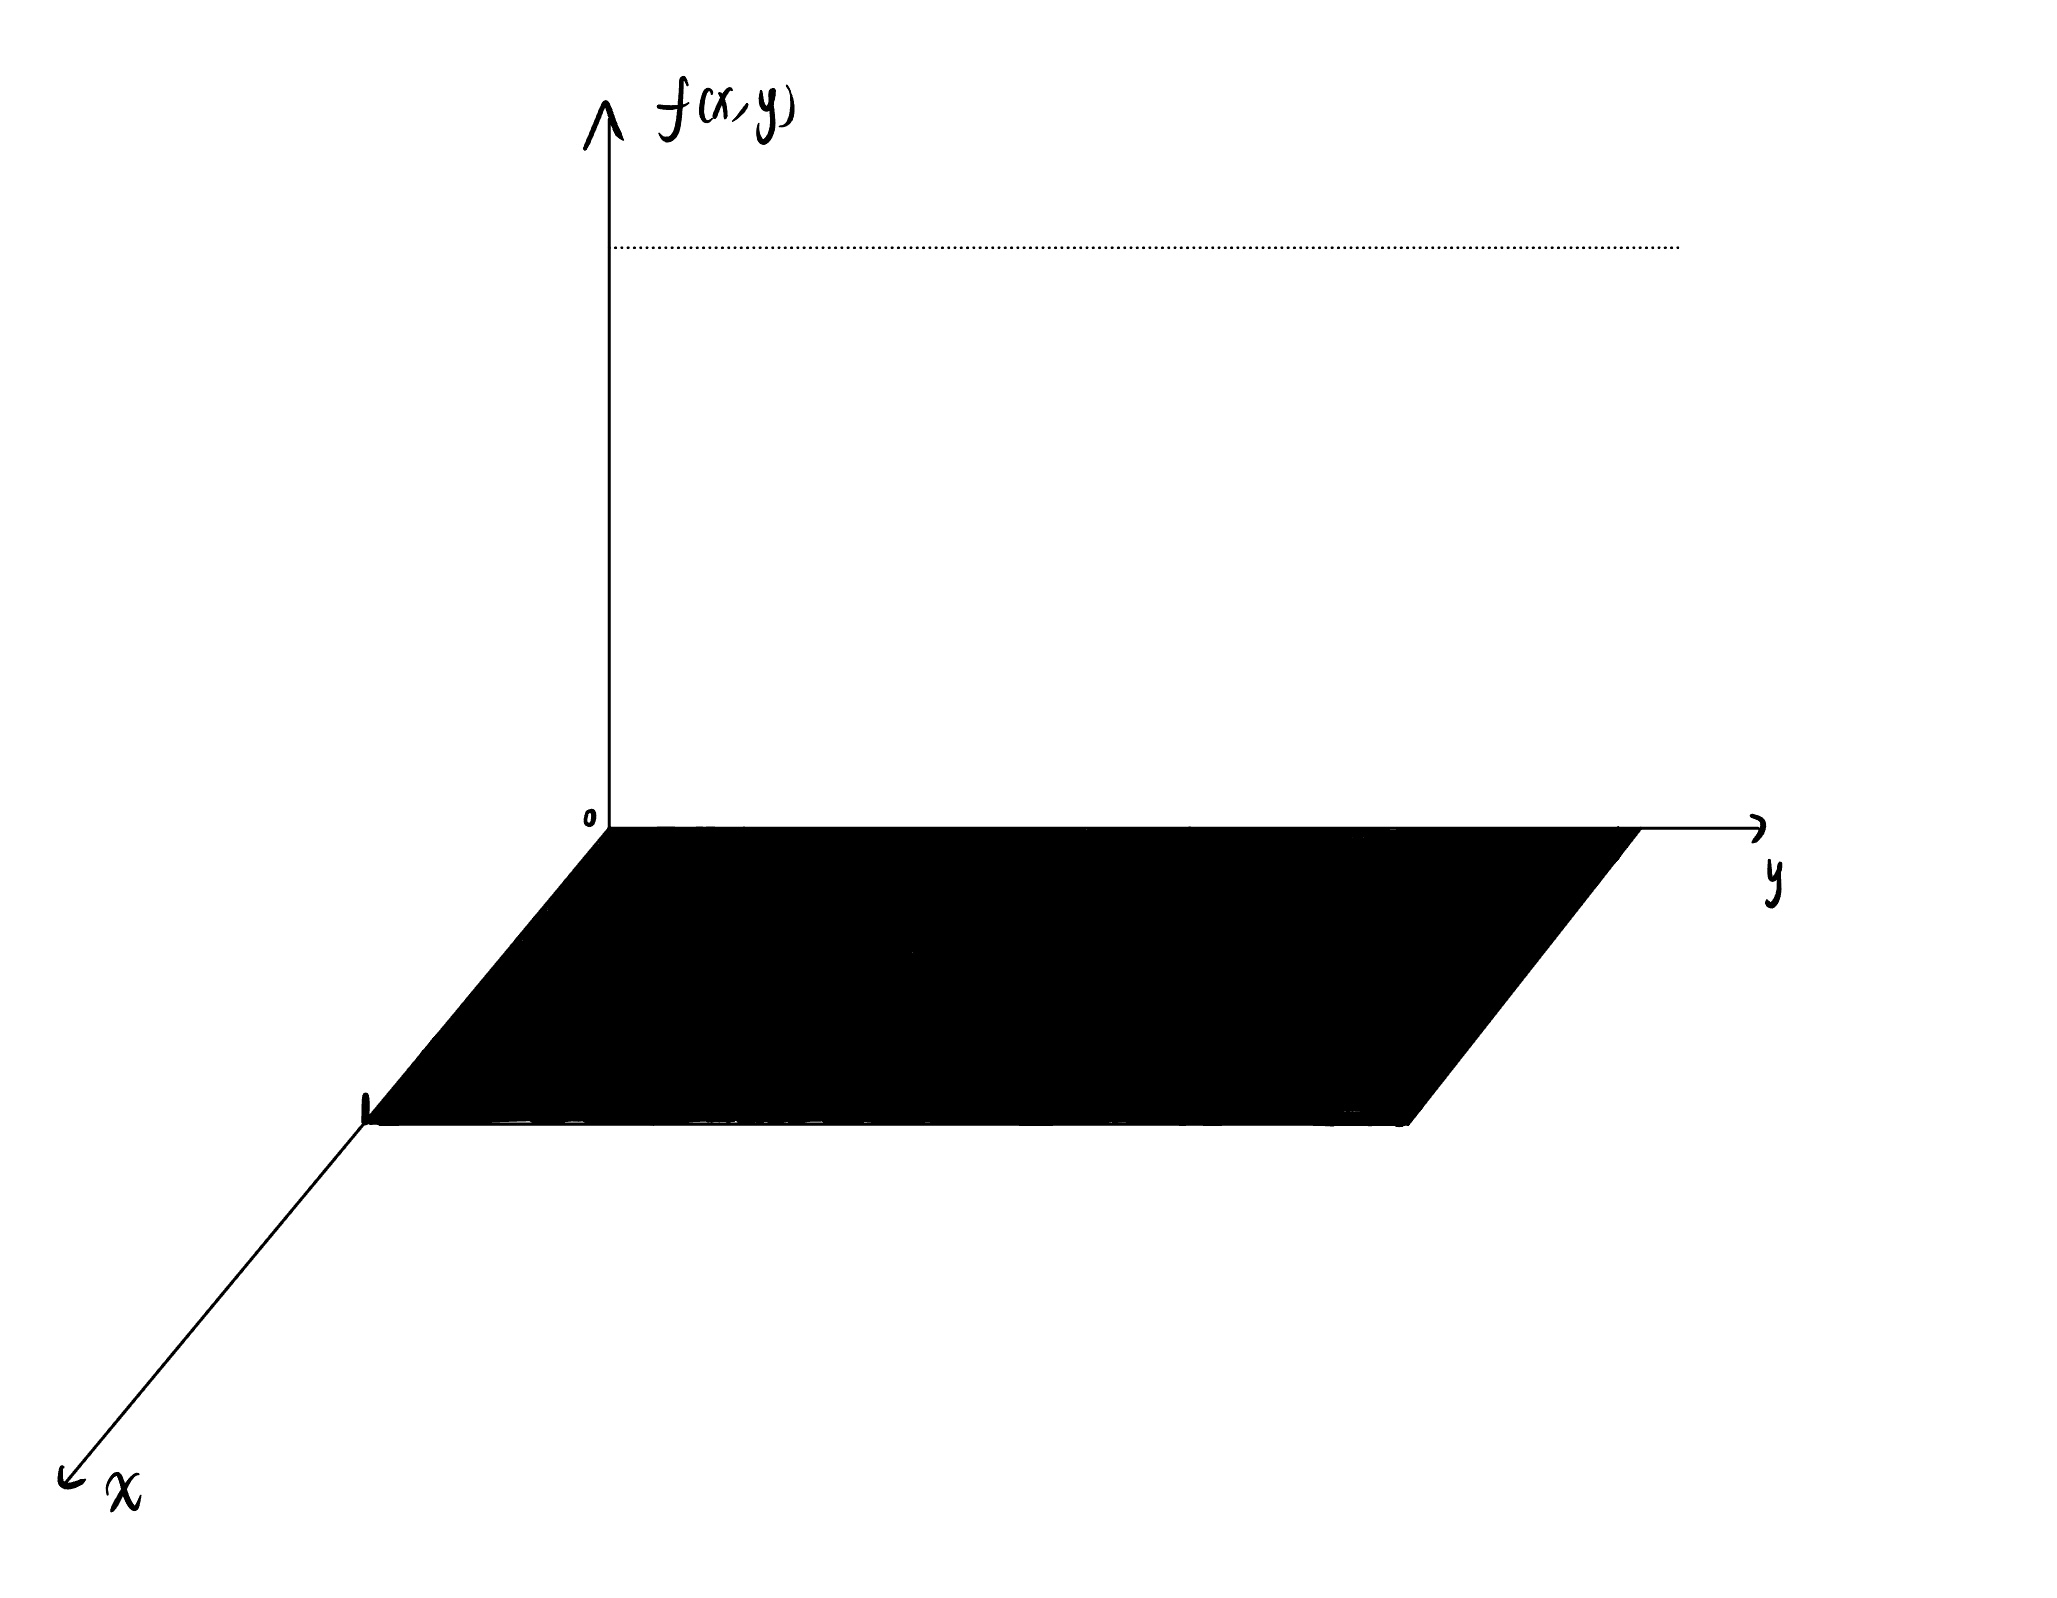
\includegraphics[scale=0.1]{images/IMG_0341.jpeg}
    \end{figure}
    It is clear that $f$ is integrable over $Q$ because the discontinuity set has measure zero. For $x=0$, $\int_{y=0}^{y=1}f(0,y)\di y$ does not exist. But the upper and lower integrals are well-defined
    $$\overline{I}(0)=\overline{\int_{y\in [0,1]}}f(0,y)=1\text{\quad and \quad}\underline{I}(0)=\underline{\int_{y\in [0,1]}}f(0,y)=0$$
    Now we notice that
    $$\int_Qf=\int_{x=0}^{x=1}\overline{I}(x)\di x=\int_{x=0}^{x=1}\underline{I}(x)\di x=0$$
    \item Actually, we can still generalize this theorem, which is the Fubini for $\R^2$.
\end{itemize}

\begin{theorem}[Fubini for $\R\times\R$]
    Let $Q=I_1\times I_2\subset \R^2$ where $I_1,I_2$ are closed intervals in $\R$. Let $f:Q\longrightarrow\R$ be bounded. 
    If $\int_Qf$ exists. For each $x$, consider the lower and upper integrals
    $$\overline{\int_{y\in I_2}}f(x,y)\text{\quad and \quad}\underline{\int_{y\in I_2}}f(x,y)$$
    These two functions of $x$ are integrable, and
    $$\int_Qf=\int_{x\in I_1}\overline{\int_{y\in I_2}}f(x,y)=\int_{x\in I_1}\underline{\int_{y\in I_2}}f(x,y)$$
\end{theorem}

\noindent \textbf{Remark}:
\begin{itemize}
    \item Before we get into the full Fubini's theorem, we will make clear the following definitions.
    \item We should keep in mind that we only defined the integral of functions from closed rectangle in $\R^n$ to $\R$.
\end{itemize}

\begin{definition}
    Let $Q=I_1\times\cdots\times I_m\times J_1\times\cdots \times J_n$ be a closed rectangle in $R^{m+n}$ where all $I_i$ and $J_k$ are closed interval. Let $Q_1=I_1\times \cdots \times I_m$ be a closed rectangle in $\R^m$ and $Q_2=J_1\times\cdots\times J_n$ be a closed rectangle in $\R^n$.
    We define
    $$Q=Q_1\times Q_2$$
    In particular, we have $$\R^{m+n}=\R^m\times \R^n$$
    Also, let $A\subset \R^m$, $B\subset\R^n$, $C\subset \R^p$ be closed rectangles, then $$(A\times B)\times C=A\times (B\times C)$$
    For $c=(x_1,\cdots,x_m,y_1,\cdots,y_n)\in \R^{m+n}$, let $x=(x_1,\cdots,x_m)\in \R^m$, $y=(y_1,\cdots,y_n)\in \R^m$, we write $$c=(x,y)\in \R^{m+n}$$
\end{definition}

\noindent \textbf{Remark}:
\begin{itemize}
    \item I admit that this is an abuse of notations. The above we defined is the product of subsets of $\R^n$, not the cartesian product of arbitrary sets.
    \item In view of set theory(cartesian product of sets), $$\R^{m+n}\neq\R^m\times\R^n$$
    But the difference is very subtle. To be precise $$\R^{m+n}=U\oplus V$$
    where $$U=\{(x_1,\cdots,x_m,0,\cdots,0):(x_1\cdots,x_m)\in \R^m\}$$
    $$V=\{(0,\cdots,0,y_1,\cdots,y_n):(y_1\cdots,y_n)\in \R^n\}$$
    The subspaces $U$ and $V$ looks exactly like $\R^m$ and $\R^n$. $U\oplus V$ and $\R^m\times \R^n$ are not only isomorphic, they are called \underline{canonically isomorphic}. It is like the relation of the vector space $V$ and its double dual space $V^{**}$.
    \item Our definition means whenever we are in spaces like $\R^{m+n}$, we can view it as a hyperplane where the two hyperlines looks exactly like $\R^m$ and $\R^n$.
\end{itemize}

\begin{theorem}[Full Fubini]
    Let $f : Q\subset\R^{m+n} \longrightarrow \R$ be a bounded function and $Q = A \times B$ a rectangle as defined above where $A\subset\R^m$ and $B\subset \R^n$.
    We write $f = f(x,y)$, where $x \in A$, and $y \in B$. Fixing $x \in A$, $f(x,y)$ is a function of $y$. Since this function is bounded, the lower and upper integrals are defined.
    $$\underline{I}(x)=\underline{\int_{y\in B}}f(x,y)$$
    $$\overline{I}(x)=\overline{\int_{y\in B}}f(x,y)$$
    Note that $\underline{I}(x) \leq \overline{I}(x)$. The Fubini Theorem concludes the following: If $f$ is integrable over $Q$, then $\underline{I}(x)$ and $\overline{I}(x)$ are integrable over $A$ and
    $$\int_Qf=\int_{x\in A}\underline{I}(x)=\int_{x\in A}\overline{I}(x)$$
\end{theorem}

\section{Riemann Integral over Bounded Sets}

\noindent \textbf{Motivation}:
\begin{itemize}
    \item In reality, we often encounter questions like computing the mass of an object $M$ which is not a simple rectangle. Given the density function $\rho(x,y,z)$, we should integrate $\rho$ over $M$.
    \item We should generalize the definition of integral over a bouded set.
\end{itemize}

\begin{definition}
    Let $S$ be a bouded set in $\R^n$. Let $f:S\longrightarrow \R$ be a bounded function. Define $f_S:\R^n\longrightarrow\R$ by the following
    \begin{equation}
        f_S(x)=
        \begin{cases}
            f(x)\text{\quad for } x\in S\\
            0\text{\quad otherwise}
        \end{cases}
    \end{equation}
    Choose a rectangle $Q$ containing $S$. We define the \underline{integral of $f$ over $S$} by the following
    \begin{equation}
        \int_Sf=\int_Qf_S
    \end{equation}
    provided the latter integral exists.
\end{definition}
\noindent \textbf{Remark}:
\begin{itemize}
    \item We must show that $\int_Sf$ is independent of the choice of $Q$.
    \item We will prove this by the following lemma.
\end{itemize}

\begin{lemma}
    Let $Q$ and $Q'$ be two rectangles in $\R^n$. Let $f:\R^n\longrightarrow\R$ be a bounded function that vanishes outside $Q\cap Q'$, then $f$ is integrable over $Q$ if and only if $f$ is integrable over $Q'$. and
    $$\int_Qf=\int_{Q'}f$$
\end{lemma}


\begin{lemma}
    Let $S\subset \R^n$. Let $f,g:S\longrightarrow \R$. Define 
    $$M=\max\{f(x),g(x)\} \text{\quad and \quad}m=\min\{f(x),g(x)\}$$ 
    Then we have:
    \begin{enumerate}
        \item If $f$ and $g$ are continuous at $x_0$, then $M$ and $m$ are also continuous at $x_0$.
        \item If $f$ and $g$ are integrable over $S$, then $M$ and $m$ are integrable over $S$.
    \end{enumerate}
\end{lemma}


\begin{theorem}[Properties of integral] \label{properties of integral}
    Let $S\subset \R^n$ be bounded. Let $f,g:\longrightarrow \R$ be bounded functions.
    \begin{enumerate}
        \item (Linearity) If $f$ and $g$ are integrable over $S$, then $af+bg$ is integrable over $S$ where $a,b$ are coefficients in $\R$. And we have the formula $$\int_S(af+bg)=a\int_Sf+b\int_Sg$$
        \item (Comparison) Suppose $f$ and $g$ are integrable over $S$.
        \begin{enumerate}
            \item If $\forall x \in S.f(x)\leq g(x)$, then $$\int_Sf\leq \int_Sg$$
            \item $|f|$ is also integrable over $S$ and $$\left|\int_Sf\right|\leq \int_S|f|$$
        \end{enumerate}
        \item (Monotonicity) Let $T\subset S$. If $f$ is non-negative on $S$ and integrable over $T$ and $S$, then $$\int_Tf\leq \int_Sf$$
        \item (Additivity) If $S=S_1\cup S_2$ and $f$ is integrable over $S_1$ and $S_2$, then $f$ is integrable over $S$ and $S_1\cap S_2$. And we have the equation $$\int_Sf=\int_{S_1}f+\int_{S_2}f-\int_{S_1\cap S_2}f$$
    \end{enumerate}
\end{theorem}


\begin{corollary}
    Let $S_1,\cdots,S_k$ be bouded sets in $\R^n$. Assume $S_i\cap S_j$ has measure zero whenever $i\neq j$. Let $S=S_1\cup\cdots\cup S_k$. If $f$ is integrable over each $S_i$, then $f$ is integrable over $S$ and $$\int_Sf=\int_{S_1}f+\cdots+\int_{S_k}f$$
\end{corollary}

\noindent \textbf{Remark}:
\begin{itemize}
    \item Our primary interest is studying the integral of the continuous function $f:S\longrightarrow\R$.
    \item By definition, we find any rectangle $Q$ containing $S$ and extend $f$ to the function $f_S:Q\longrightarrow\R$, then it is reduced to the integral over a rectangle. We know that $f_S$ is integralable over $Q$ iff the set of points $D$ where $f_S$ fails to be continuous has measure zero.
    \item When $f:S\longrightarrow\R$ is continuous, the set $D$ should be in the boundary of $S$. So it is convenient for us to find conditions of $S$ in order to make $f$ integrable over $S$.
\end{itemize}

\begin{theorem}\label{f integrable over S iff E has measure zero}
    Let $S$ be a bounded set in $\R^n$. Let $f:S\longrightarrow\R$ be a bounded continuous function. Let $E$ be the set of points $x_0$ of $Bd(S)$ such that $$\lim_{x\to x_0}f(x)\neq 0$$
    $E$ has measure zero if and only if $f$ is integrable over $S$.
\end{theorem}

\begin{theorem}\label{integral over interior}
    Let $S$ be a bounded set in $\R^n$. Let $f:S\longrightarrow \R$ be a bounded continuous function. Let $A=Int(S)$. If $f$ is integrable over $S$, then $f$ is integrable over $A$ and $$\int_Sf=\int_Af$$
\end{theorem}


\begin{theorem*}
    Let $S$ be a bounded set in $\R^n$. Let $f:S\longrightarrow\R$ be a bounded function. Let $D$ be the set of points of $S$ at which $f$ fails to be continuous. Let $E$ be the set of points of $Bd(S)$ at which $$\lim_{x\to x_0}f(x)\neq0$$
    Then $\int_Sf$ exists if and only if $D$ and $E$ have measure zero.
\end{theorem*}
\noindent \textbf{Remark}:
\begin{itemize}
    \item We proved this in homework.
\end{itemize}

\section{Rectifiable Sets}

\begin{definition}
    A bounded set $S\subset \R^n$ is called \underline{rectifiable} (Only for this book) if and only if  the characteristic function 
    \begin{equation}
        \chi_S(x)=\begin{cases}
            1 \text{\quad}x\in S\\
            0 \text{\quad}x\notin S
        \end{cases}
    \end{equation} is integrable. And we define the \underline{(n-dimensional) volume} of $S$ by the equation $$v(S)=\int_S1$$
\end{definition}
\noindent \textbf{Remark}:
\begin{itemize}
    \item The volume is also called \underline{(Jordan) content}
\end{itemize}

\begin{theorem}
    $S\subset \R^n$ is rectifiable if and only if $S$ is bounded and $Bd(S)$ has measure zero.
\end{theorem}
\noindent \textbf{Remark}:
\begin{itemize}
    \item We can see that this theorem is actually a corollary of theorem\ref{f integrable over S iff E has measure zero}.
    \item Theorem\ref{f integrable over S iff E has measure zero} says that given $S$ and $f$, we can check whether $f$ is integrable over $S$. This theorem tells us if $S$ is a rectifiable set, then any continuous bounded function $f$ is integrable over $S$.
    \item I call the rectifiable set $S$ the set at which we can do integration without worries.
\end{itemize}

\noindent \textbf{Example}: Example of bounded set that is not rectifiable.
\begin{itemize}
    \item Define $S=\{p\in \R: p\in \Q \text{ and }p\in (0,1)\}$. We proved in MAT157 that $S$ is countable. So we can write $S$ as $S=\{p_1,p_2,p_3,\cdots\}$ with $p_i<p_{i+1}$. 
    Let $0<a<1$ be given. For each $p_i$, we can choose an open interval $(a_i,b_i)$ of length less than $\frac{a}{2^i}$ that contains $p_i$ and contained in $(0,1)$. Define $$A=\bigcup_{i=1}^{\infty}(a_i,b_i)$$
    We can show $Bd(A)$ does not have measure zero, so $A$ is an bounded open set that is not rectifiable.
\end{itemize}

\begin{theorem}[Properties of rectifiable sets] \label{properties of rectifiable sets}\
    \begin{enumerate}
        \item (Positivity) If $S$ is rectifiable, then $v(S)\geq 0$.
        \item (Monotonicity) If $S_1,S_2$ are rectifiable with $S_1\subset S_2$, then $v(S_1)\leq v(S_2)$.
        \item (Additivity) If $S_1$ and $S_2$ are rectifiable, then $S_1\cup S_2$ and $S_1\cap S_2$ are rectifiable, and $$v(S_1\cup S_2)=v(S_1)+v(S_2)-v(S_1\cap S_2)$$
        \item Suppose $S$ is rectifiable. Then $v(S)=0$ if and only if $S$ has measure zero.
        \item Suppose $S$ is rectifiable, then $Int(S)$ is also rectifiable and $v(S)=v(Int(S))$.
        \item Suppose $S$ is rectifiable. Then if $f:S\longrightarrow\R$ is bounded and continuous, then $f$ is integrable over $S$.
    \end{enumerate}
\end{theorem}

\begin{definition}
    Let $C$ be a compact and rectifiable set in $\R^{n-1}$. Let $\phi,\psi:C\longrightarrow\R$ be continuous functions such that $\forall x\in C. \phi(x)\leq \psi(x)$. The subset $S\subset \R^n$ defined by the equation
    $$S=\{(x,t): x\in C \text{ and }\phi(x)\leq t \leq \psi(x)\}$$ is called a \underline{simple region} in $\R^n$.
    \begin{figure}[ht]
        \centering
        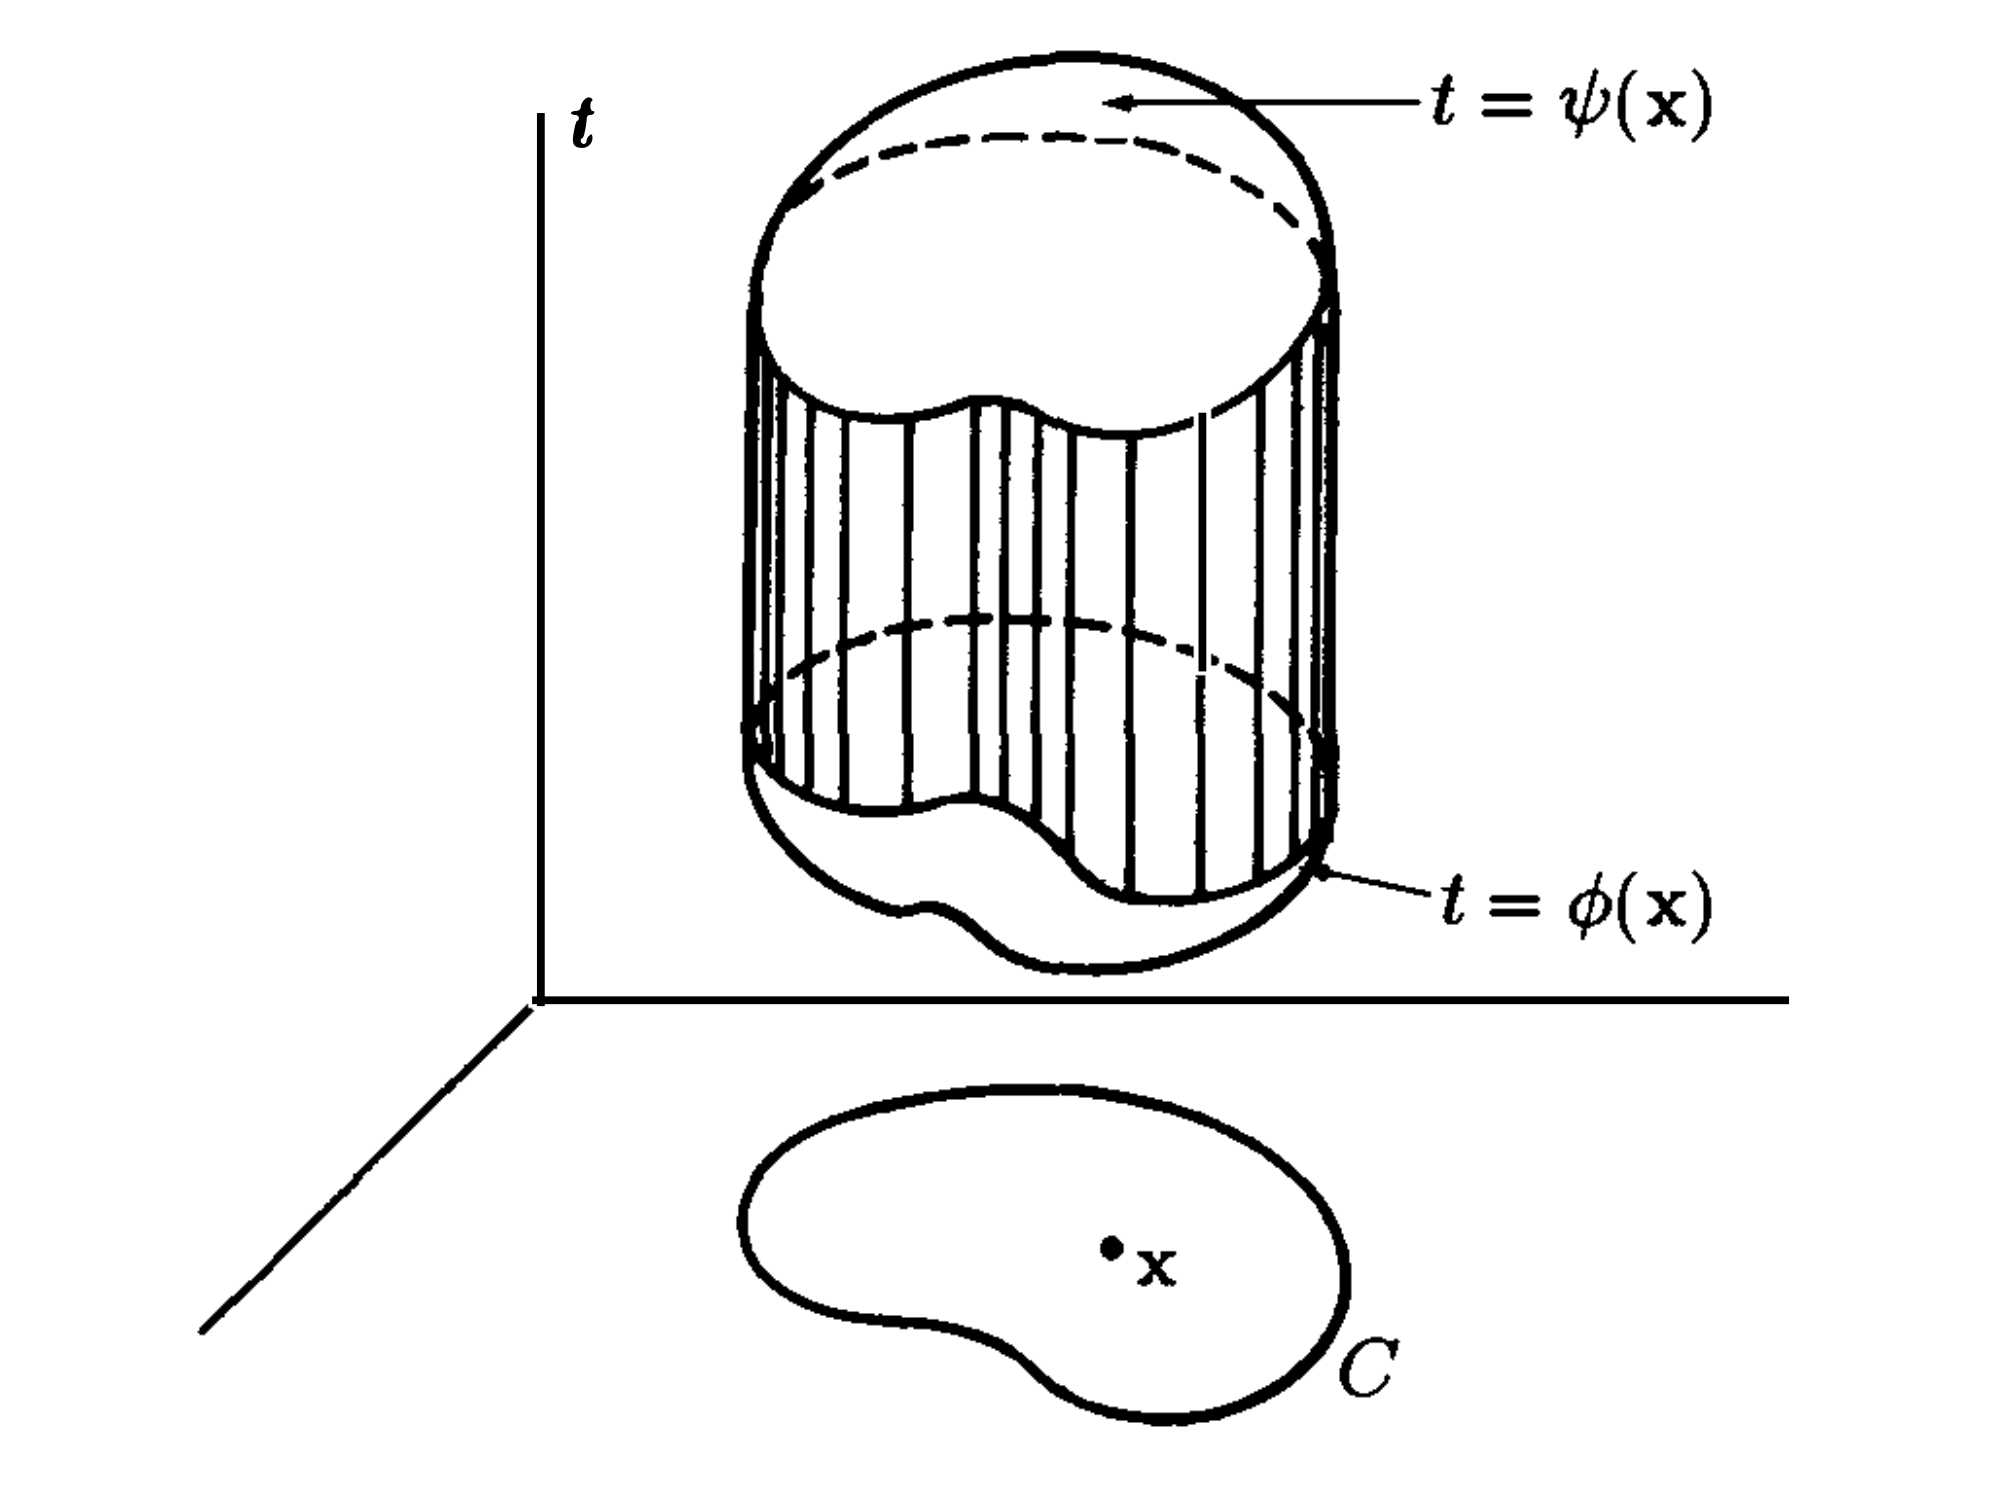
\includegraphics[scale=0.3]{images/Screenshot 2022-11-14 at 17.42.56.png}
        \caption{A picture of simple region in $\R^3$}
    \end{figure}
\end{definition}

\begin{lemma}
    If $S$ is a simple region in $\R^n$, then $S$ is compact and rectifiable.
\end{lemma}

\begin{theorem}[Fubini for simple region]\label{fubini for simple region}
    Let $S$ be a simple region in $\R^n$
    $$S=\{(x,t): x\in C \text{ and }\phi(x)\leq t \leq \psi(x)\}$$
    Let $f:S\longrightarrow\R$ be a continuous function. Then $f$ is integrable over $S$ and $$\int_Sf=\int_C\int_{t=\phi(x)}^{t=\psi(x)}f(x,t)$$
\end{theorem}
\noindent \textbf{Remark}:
\begin{itemize}
    \item This theorem gives us a reasonable method for reducing the n-dimensional integral $\int_Sf$ to lower-dimensional integrals. If $C$ is simple, we can apply this theorem again.
    \item If $S$ is not simple, one can try to exprss $S$ as a union of simple regions that overlap insets of measure zero.
\end{itemize}

\noindent \textbf{Example}:
\begin{itemize}
    \item Consider the set $S=\{(x,y):1\leq x^2+y^2\leq 4\}$.
    \begin{figure}[ht]
        \centering
        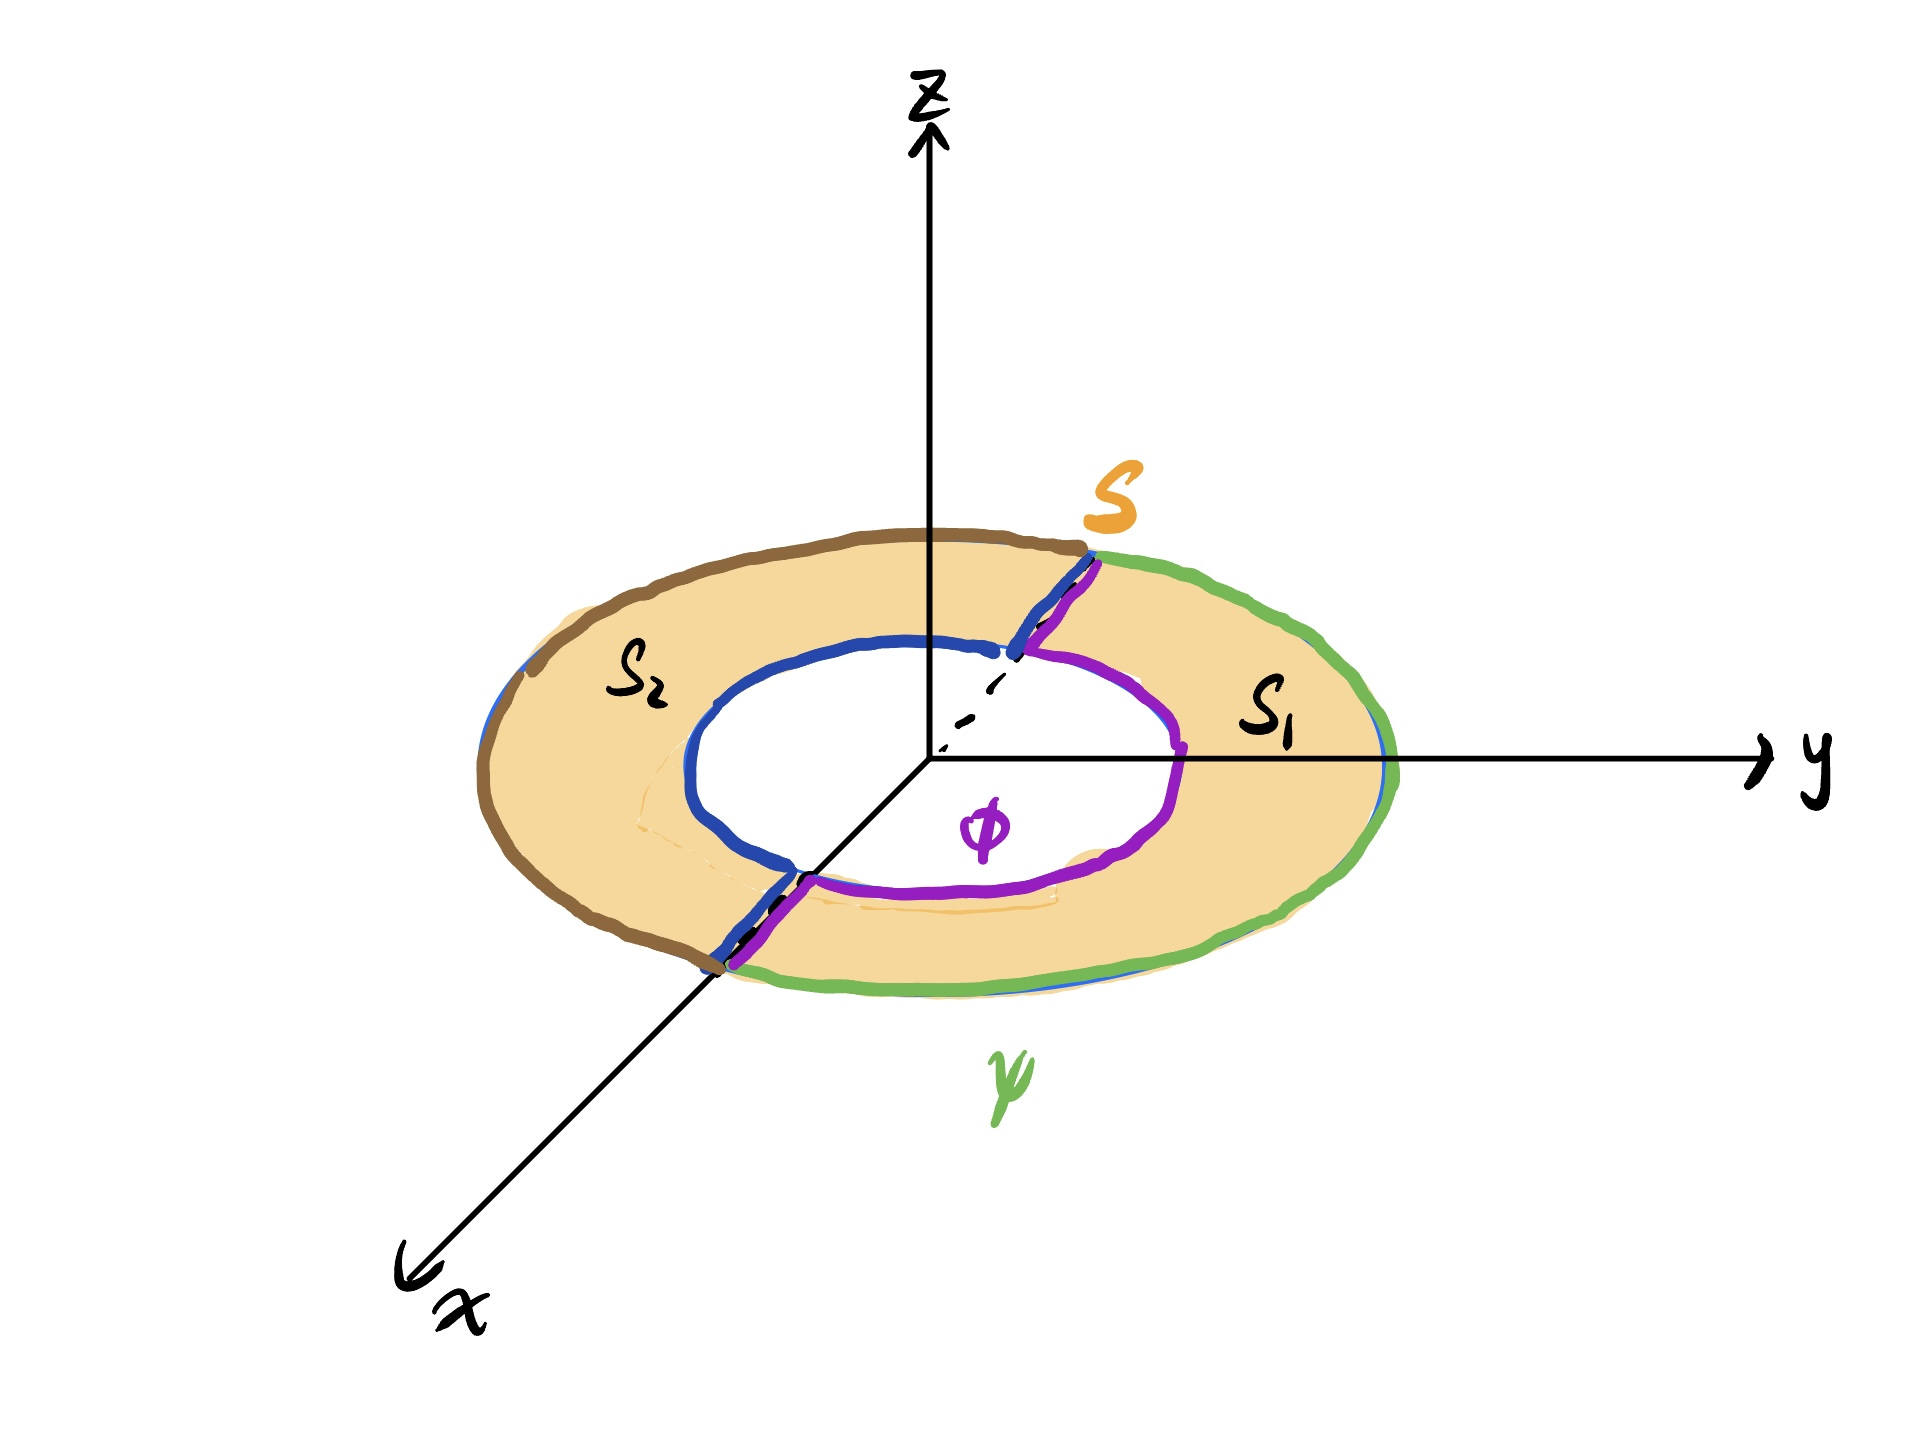
\includegraphics[scale=0.15]{images/IMG_0355.jpg}
        \caption{A picture of $S=\{(x,y):1\leq x^2+y^2\leq 4\}$}
    \end{figure}
    What we want to do is to compute the (Jordan)content of $S$. While $S$ is not a simple region, one can evaluate an integral over $S$ by breaking $S$ up into two simple regions $S_1,S_2$ that overlap in a set of measure zero, as indicated, and integrating over each of these regions separately. Define 
    $$C=[-2,2]$$
    $$\phi(x)=\begin{cases}
        0\text{\quad}x\in[-2,-1]\cup[1,2]\\
        \sqrt{1-x^2}\text{\quad}x\in(-1,1)
    \end{cases}$$
    $$\psi(x)=\sqrt{4-x^2}\text{\quad}x\in C$$
    $$S_1=\{(x,t):x\in C \text{ and }\phi(x)\leq t \leq \psi(x)\}$$
    Since $S_1$ is a simple region, we can apply theorem\ref{fubini for simple region}.
    \begin{equation}
        \begin{split}
            \int_{S_1}1&= \int_C \int_{t=\phi(x)}^{t=\psi(x)}1\\
            &= \int_C t\big|_{\phi(x)}^{\psi(x)}\\
            &= \int_C(\psi(x)-\phi(x))\\
            &= \int_{[-2,2]}\sqrt{4-x^2}-\int_{(-1,1)}\sqrt{1-x^2}\\
            &= 2\pi-\frac{1}{2}\pi\\
            &=\frac{3}{2}\pi
        \end{split}
    \end{equation}
    Similarly, we can compute $$\int_{S_2}1=\frac{3}{2}\pi$$
    Therfore $$\int_S1=\int_{S_1}1+\int_{S_2}1=3\pi$$
    If we encounter a more complex function $f$, and want to integrate $f$ over $S$, another way is to to express the integral in terms of polar coordinates. 
    Expressing a two-dimensional integral in terms of polar coordinates is a special case of a quite general method for evaluating integrals, which is called \underline{substitution} or \underline{change of variables}. We shall deal with it in the next chapter.
\end{itemize}

\section{Improper Integral}

\noindent \textbf{Motivation}:
\begin{itemize}
    \item Up to now, we have studied integrals of bounded functions $f:S\longrightarrow\R$ over bounded sets $S\subset \R^n$.
    \item This is clearly not enough, in this section, we will extend our definition of integral to continuous functions (may not be bounded) $f:A\longrightarrow\R$ to open sets (may not be bounded) $A\subset\R^n$.
\end{itemize}

\begin{definition}
    Let $A\subset\R^n$ be open. Let $f:A\longrightarrow\R$ be continuous. If $f$ is non-negative, i.e.$$\forall x \in A.f(x)\geq0$$
    we define the \underline{(extended) integral} of $f$ over $A$ as $$\int_Af=\sup_{D\subset A}\int_Df$$
    where $D$ is a compact rectifiable subset of $A$, provided this supremum exists. In this case, we say $f$ is \underline{integrable} over $A$ (in the extended sence).
\end{definition}

\begin{definition}
    Generalize the definition above, if $f$ is an arbitrary continuous function over $A$, we consider the non-positive and non-negative parts seperately and turn them into non-negative
    $$f_+(x)=\max\{f(x),0\}$$
    $$f_-(x)=\max\{-f(x),0\}$$
    We say $f$ is \underline{integrable} over $A$  (in the extended sence) if both $\int_Af_+$ and $\int_Af_-$ exist. In this case, we set $$\int_Af=\int_Af_+-\int_Af_-$$
\end{definition}

\noindent \textbf{Remark}:
\begin{itemize}
    \item For $A$ is open and bounded, we now have two definitions of integration. But don't worry, it turns out that if the ordinary integral exists, then the extended integral and the ordinary integral are equal.
    \item But we should notice that sometimes the extended integral exists but the ordinary integral does not. So the extended integral is a more general definition. From now on, $\int_Af$ will denote the extended integral unless specifically stated otherwise.
    \item When $A$ is open in $\R$, this definition of integral is different from the improper integral of single-variable. We show this in the following example.
\end{itemize}

\begin{definition}[Improper integral of single-variable]
    Suppose the restriction of $f:(a,b)\longrightarrow\R$ to any closed subinterval is bounded and integrable. Then we define the \underline{improper integral}:
    $$\int_a^bf=\lim_{x\to a^+}\int_x^cf+\lim_{x\to b^-}\int_c^xf$$
    for any $c\in(a,b)$ provided both limits on right hand exist.
\end{definition}

\noindent \textbf{Example}:
\begin{itemize}
    \item Consider the continuous function $f:(0,\infty)\longrightarrow\R$ defined by $$f(x)=\frac{\sin(x)}{x}$$
    \begin{figure}[ht]
        \centering
        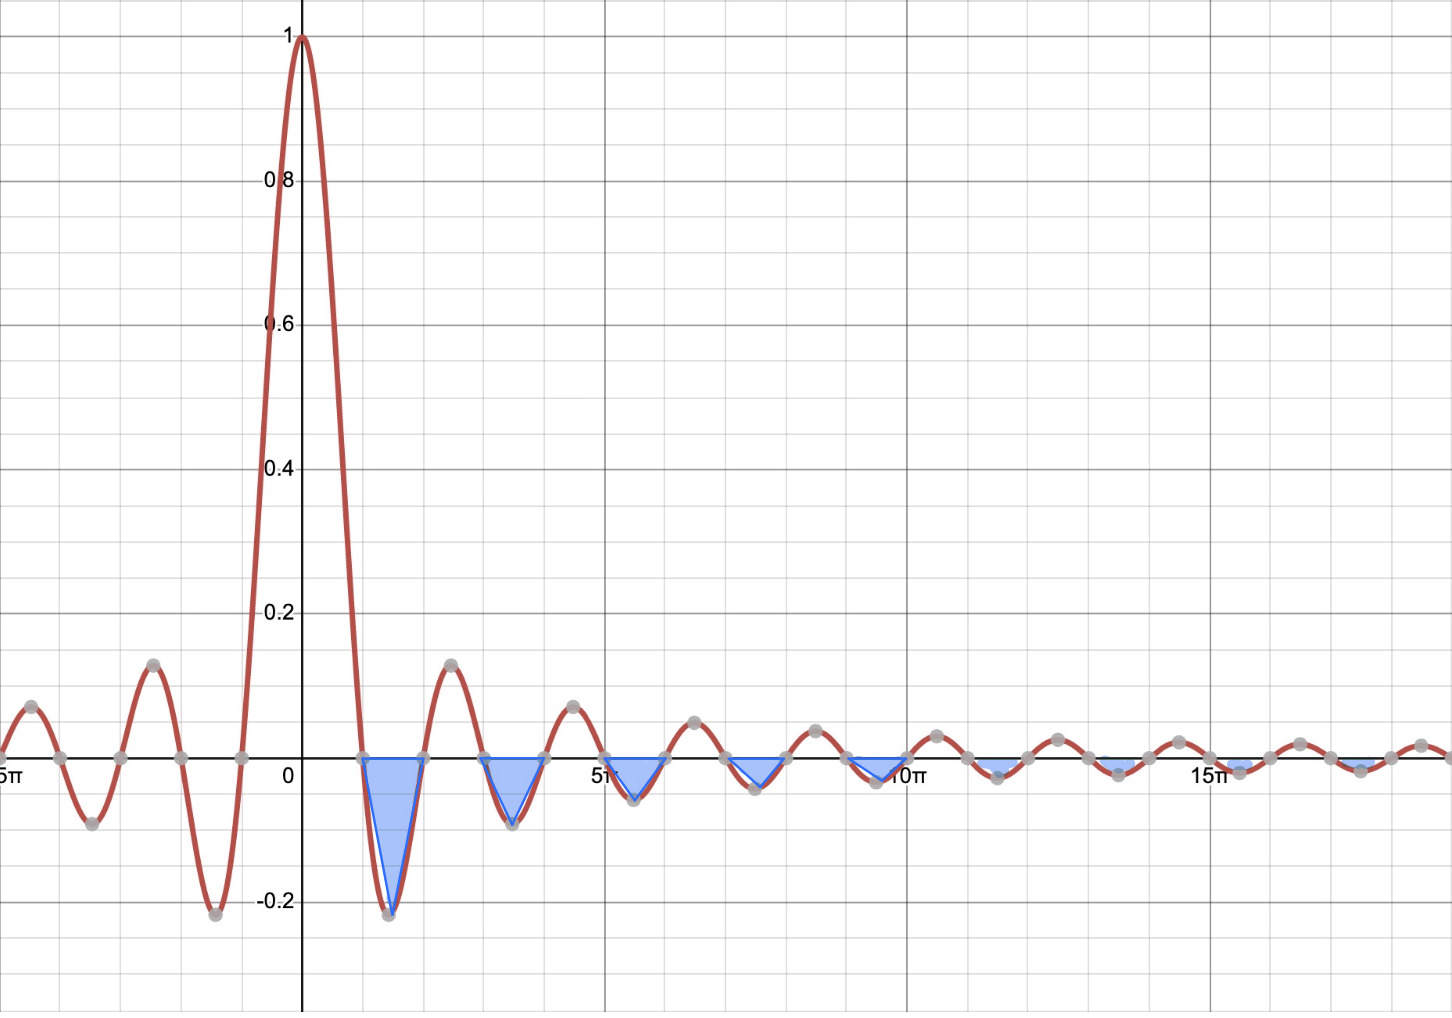
\includegraphics[scale=0.4]{images/Screenshot 2022-11-28 at 04.10.31.png}
        \caption{$f(x)=\frac{\sin(x)}{x}$}
    \end{figure}
    By the definition of improper integral of single-variable, $$\int_0^{\infty}\frac{\sin(x)}{x}\di x=\lim_{a\to 0}\int_{a}^1\frac{\sin(x)}{x}\di x+\lim_{b\to \infty}\int_1^b\frac{\sin(x)}{x}\di x$$
    The first part of RHS exists because for $0<x<1$ $$0<\frac{\sin(x)}{x}<1$$
    The second part of RHS also exists because by integration by parts
    \begin{equation}
        \begin{split}
            \lim_{b\to \infty}\int_1^b\frac{\sin(x)}{x}\di x &= \lim_{b\to \infty}\int_1^b\frac{1}{x}(-\cos(x))'\di x\\
        &= \lim_{b\to \infty}\left(\frac{1}{x}(-\cos(x))\right)\Big|_1^b-\lim_{b\to \infty}\int_1^b\frac{-1}{x^2}\cos(x)\di x\\
        &= \lim_{b \to \infty}\int_1^b\frac{1}{x^2}\cos(x)\di x-\lim_{b \to \infty}\frac{cos(b)}{b}+\cos(1)\\
        & \leq \lim_{b\to \infty}\int_1^b\frac{1}{x^2}\di x-0+cos(1)\\
        &<\infty
        \end{split}
    \end{equation}
    Therefor, the improper integral of $f$ over $(0,\infty)$ exists. Actually, it is equal to $\frac{\pi}{2}$.
    \item For $f$ defined as above. By our definition of (extended) integral, $\int_0^{\infty}\frac{\sin(x)}{x}\di x$ does not exist. Consider $$f_-(x)=\max\left\{-\frac{\sin(x)}{x},0\right\}$$
    It suffices to show that the extended integral of $f_-$ over $(0,\infty)$ does not exist. 
    Intuitively, we want to show that the extended integral of $f_-$ over $(0,\infty)$ is large than the area of these blue triangles.
    \begin{equation}
        f_-(x)=\begin{cases}
            -f(x)\text{\quad }x\in[\pi+2k\pi,2\pi+2k\pi]\\
            0 \text{\quad otherwise}
        \end{cases}
    \end{equation}
    Let us define the function of the triangles formally.
    \begin{equation}
        g(x)=\begin{cases}
            \frac{-f(\frac{3}{2}\pi+2k\pi)}{\frac{\pi}{2}}(x-\pi-2k\pi)\text{\quad}x\in[\pi+2k\pi,\frac{3}{2}\pi+2k\pi]\\
            \frac{f(\frac{3}{2}\pi+2k\pi)}{\frac{\pi}{2}}(x-2\pi-2k\pi)\text{\quad}x\in[\frac{3}{2}\pi+2k\pi,2\pi+2k\pi]\\
            0 \text{\quad otherwise}
        \end{cases}
    \end{equation}
    By our construction, $f_-(x)\geq g(x)$ for all $x\in (0,\infty)$. Let $\{C_N\}$ be an exhaustion (which we will defined below) of $(0,\infty)$ defined by $$C_N=[0+\frac{1}{N},2\pi N]$$
    So we have
    \begin{equation}
        \begin{split}
            \lim_{N\to \infty}\int_{C_N}f_-(x) &\geq \lim_{N\to \infty}\int_{C_N}g(x)\\
            &= \lim_{N\to \infty}\sum_{k=0}^{N-1}\frac{1}{2}\cdot \pi\cdot [-f(\frac{3}{2}\pi+2k\pi)]\\
            &= \lim_{N\to \infty}\sum_{k=0}^{N-1}\frac{\pi}{2}\cdot\frac{1}{\frac{3}{2}\pi+2k\pi}\\
            &= \lim_{N\to \infty}\sum_{k=0}^{N-1}\frac{1}{3+4k}\\
            &= \infty
        \end{split}
    \end{equation}
    The last step holds by the integral test. Hence $\sup_D\int_{(0,\infty)}f_-=\infty$, the supremum does not exist. 
    By the definition of extended integral of $f$ over $(0,\infty)$. It is not integrable.
\end{itemize}

\begin{theorem}\label{exhaustion}
    Let $A$ be an open set in $\R^n$. Then there exists a sequence $C_1,C_2,\cdots$ of compact rectifiable subsets of $A$ whose union is $A$, such that 
    \begin{itemize}
        \item $C_N\subset Int(C_{N+1})$
        \item $\bigcup C_N=A$
    \end{itemize}
\end{theorem}


\begin{definition}
    The sequence of sets $\{C_N\}$ in theorem\ref{exhaustion} is called an \underline{exhaustion} of $A$.
\end{definition}

\begin{theorem}[Equivalent definition of extended intrgral 1]\label{Equivalent definition of extended intrgral 1}
    Let $A\subset\R^n$ be open. Let $f:A\longrightarrow\R$ be continuous. Choose an exhaustion $\{C_N\}$ of $A$. Then $f$ is integrable over $A$ if and only if the sequence $\int_{C_N}|f|$ is bounded. In this case $$\int_Af=\lim_{N\to \infty}\int_{C_N}f$$
\end{theorem}

\begin{corollary}
    Let $A\subset\R^n$ be open. Let $f:A\longrightarrow\R$ be continuous. Then the extended integral of $f$ over $A$ exists if and only if the extended integral of $|f|$ over $A$ exists.
\end{corollary}

\begin{theorem}[Properties of extended integral]\label{Properties of extended integral}
    Let $A\subset\R^n$ be open. Let $f,g:A\longrightarrow\R$ be continuous.
    \begin{enumerate}
        \item (Linearity) If $f$ and $g$ are integrable over $A$, so is $af+bg$, and
        $$\int_A(af+bg)=a\int_Af+b\int_Ag$$
        \item (Comparision) Let $f,g$ be integrable over $A$.
        \begin{enumerate}
            \item If $f(x)\leq g(X)$ for all $x\in A$, then $$\int_Af\leq \int_Ag$$
            \item $|f|$ is also integrable over $A$ and $$\big|\int_Af\big|\leq \int_A|f|$$
        \end{enumerate}
        \item (Monotonicity) Assume $B$ is open and $B\subset A$. If $f$ is non-negative on $A$ and integrable over $A$, then $f$ is integrable over $B$ and $$\int_Bf\leq\int_Af$$
        \item (Additivity) Suppose $A$ and $B$ are open in $R^n$ and $f$ is continuous on $A\cup B$. If $f$ is integrable on $A$ and $B$, then $f$ is integrable on $A\cup B$ and $A \cap B$ and $$\int_{A\cup B}f=\int_Af+\int_Bf-\int_{A\cap B}f$$
    \end{enumerate}
\end{theorem}

\begin{theorem}[Relation between ordinary and extended integrals]
    Let $A$ be a bounded open set in $\R^n$. Let $f:A\longrightarrow \R$ be a bounded continuous function. Then the extended integral $\int_Af$ exist. 
    If the ordinary integral $\int_Af$ also exists, then these two integrals are equal.
\end{theorem}

\begin{corollary}
    Let $S$ be a bounded set in $\R^n$. Let $f:S\longrightarrow \R$ be a bounded continuous function. If $f$ is integrable over $S$ in the ordinary sense, then $$\text{(ordinary) }\int_Sf=\text{(extended) }\int_Sf$$
\end{corollary}

\begin{theorem}[Equivalent definition of extended intrgral 2]\label{Equivalent definition of extended intrgral 2}
    Let $A$ be open in $\R^n$. Let $f:A\longrightarrow \R$ be continuous. Let $U_1\subset U_2\subset U_3\subset \cdots$ be a sequence of open sets whose union is $A$. Then $\int_Af$ exists if and only if the sequence $\int_{U_N}|f|$ exists and is bounded. In this case, $$
    \int_Af=\lim_{N\to\infty}\int_{U_N}f$$
\end{theorem}

\noindent \textbf{Examples}:
\begin{itemize}
    \item Let $A=\{(x,y):x>1\text{ and }y>1\}\subset \R^2$, let $f(x,y)=\frac{1}{x^2y^2}$. Is $f$ integrable over $A$ in the extended sense? Compute the integral.
    \begin{figure}[ht]
        \centering
        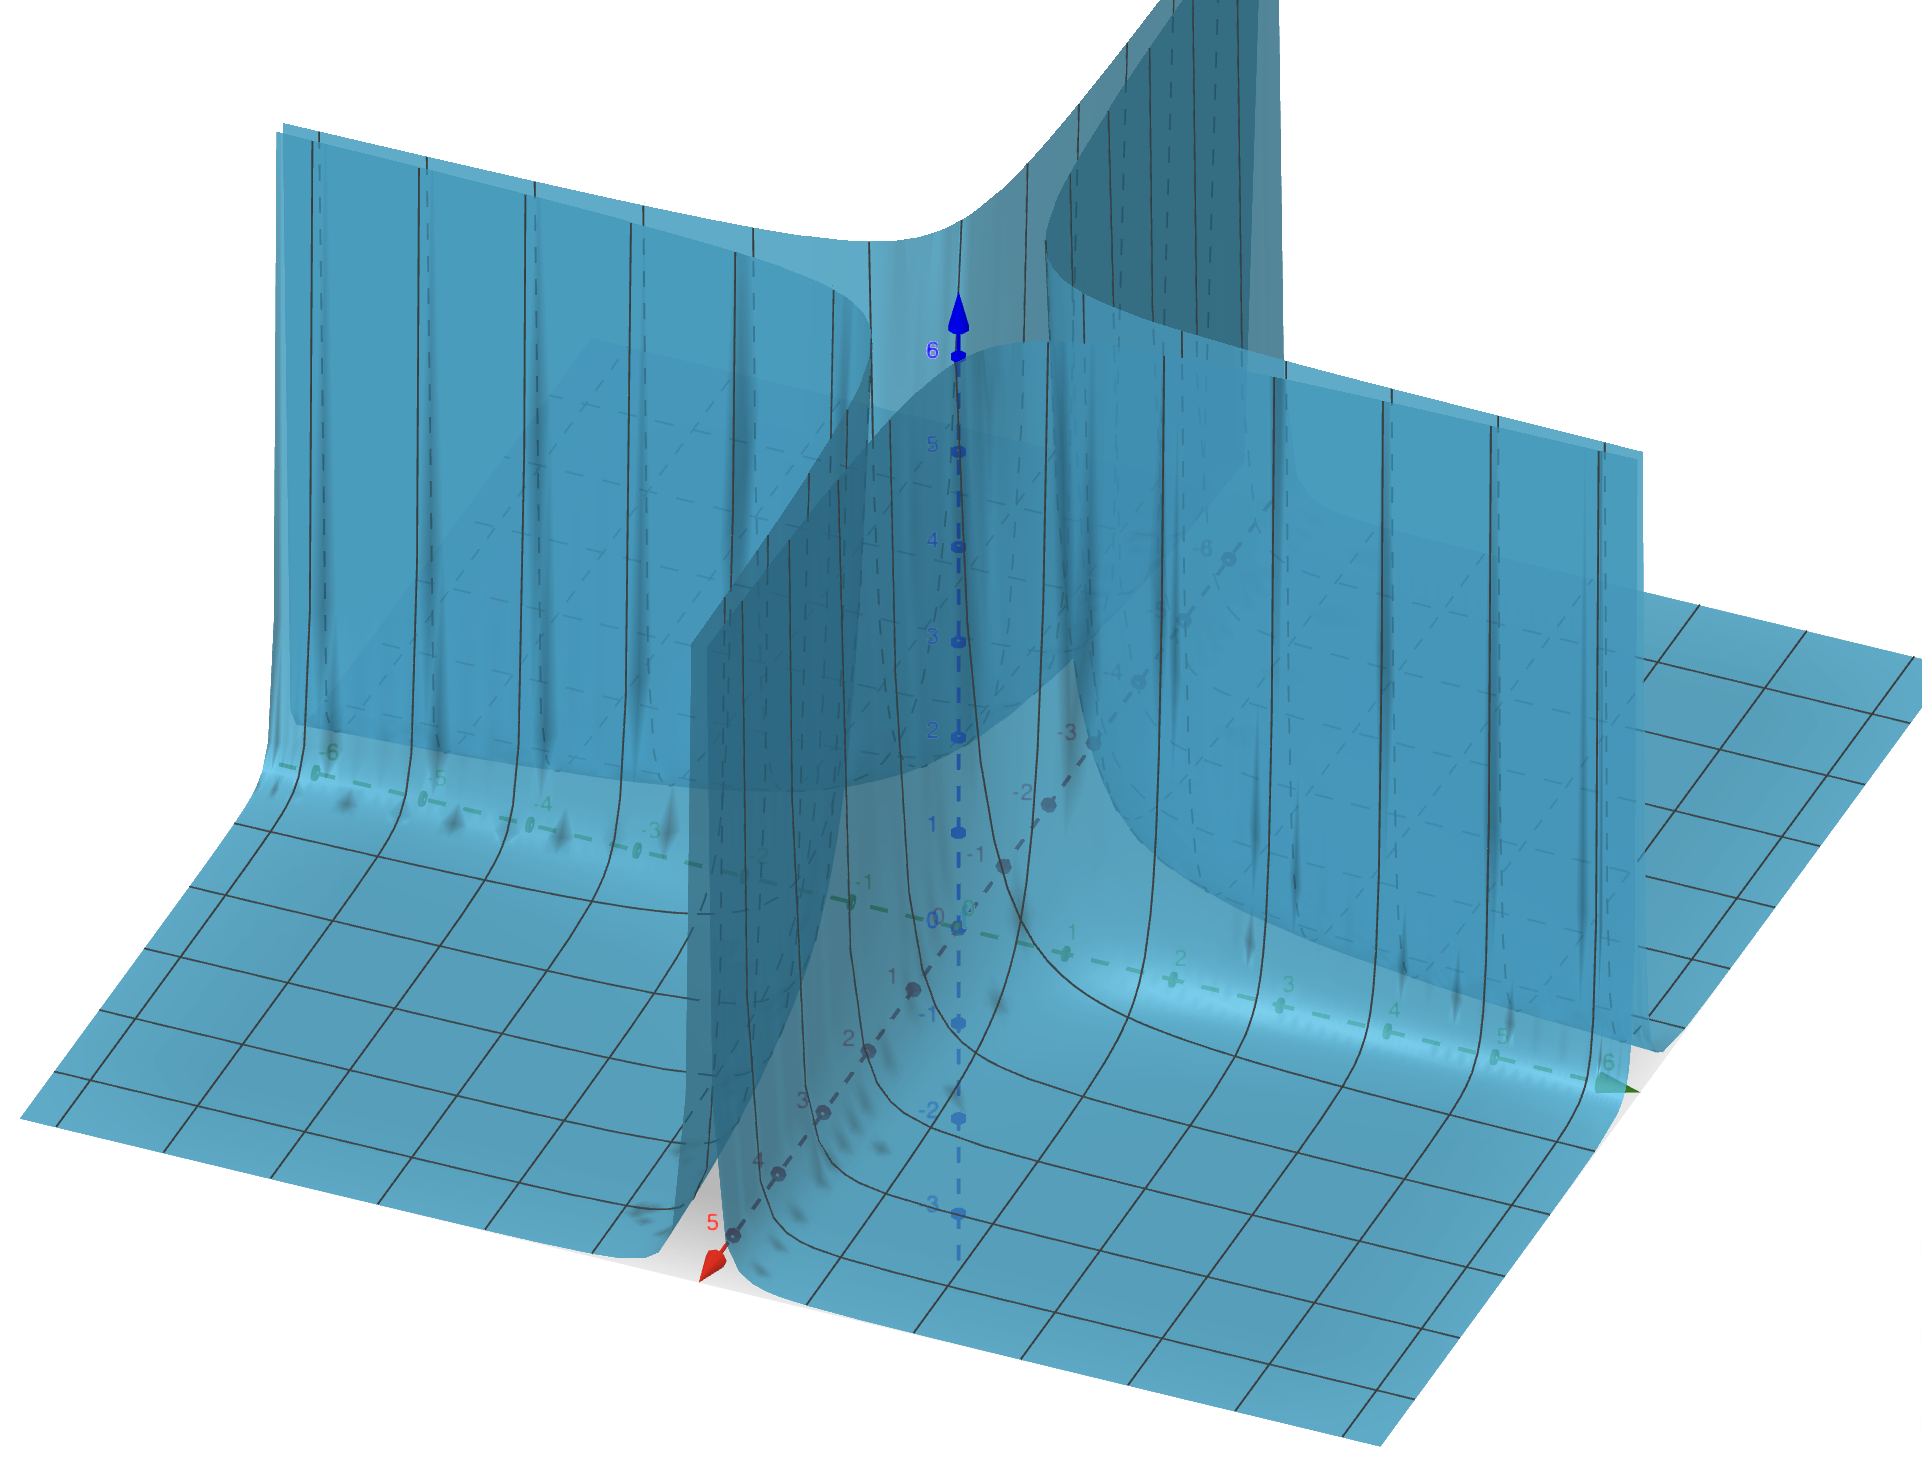
\includegraphics[scale=0.25]{images/Screenshot 2023-01-04 at 18.10.14.png}
        \caption{picture of $f(x,y)=\frac{1}{x^2y^2}$}
    \end{figure}
    \begin{enumerate}
        \item We can use theorem\ref{Equivalent definition of extended intrgral 1} to compute. Set $$C_N=[\frac{N+1}{N},N]^2$$
        Firstly, we need to show the sequence $\int_{C_N}|f|$ is bounded.
        \begin{equation}
            \begin{split}
                \int_{C_N}|f| &= \int_{C_N}f\\
                &= \int_{x\in[\frac{N+1}{N},N]}\int_{y\in[{\frac{N+1}{N},N}]}\frac{1}{x^2y^2}\di y\di x\\
                &= \int_{x\in[\frac{N+1}{N},N]}\left(\frac{-1}{x^2}\cdot \frac{1}{y}\right) \bigg\rvert_{\frac{N+1}{N}}^N\di x\\
                &= \int_{x\in[\frac{N+1}{N},N]}(\frac{N}{N+1}-\frac{1}{N})\frac{1}{x^2}\di x\\
                &= (\frac{N}{N+1}-\frac{1}{N})\frac{-1}{x} \bigg\rvert_{\frac{N+1}{N}}^N\\
                &= (\frac{N}{N+1}-\frac{1}{N})^2
            \end{split}
        \end{equation}
        Taking the limit we have $$\lim_{N\to\infty}(\frac{N}{N+1}-\frac{1}{N})^2=1$$
        So $f$ is integrable over $A$.
        \begin{equation}
            \begin{split}
                \int_Af &= \lim_{N\to\infty}\int_{C_N}f\\
                &= \lim_{N\to\infty}(\frac{N}{N+1}-\frac{1}{N})^2\\
                &= 1
            \end{split}
        \end{equation}
        \item It is easier for us to use theorem\ref{Equivalent definition of extended intrgral 2} to solve this problem.
        Set $$U_N=(1,N)^2$$
        Can check that $U_1\subset U_2\subset\cdots$ and $\bigcup_{N=1}^{\infty}U_N=A$. By theorem\ref{f integrable over S iff E has measure zero}, $E=Bd(\overline{U_N})$ has measure zero, so $f$ is integrable over $\overline{U_N}$.
        By theorem\ref{integral over interior}, $\int_{U_N}f=\int_{\overline{U_N}}f$.
        \begin{equation}
            \begin{split}
                \int_{U_N}|f| &= \int_{\overline{U_N}}f\\
                &= \int_{x\in[1,N]}\int_{y\in[1,N]}\frac{1}{x^2y^2}\di y\di x\\
                &= \int_{x\in[1,N]}(\frac{-1}{x^2}\cdot\frac{1}{y}) \bigg\rvert_1^N\di x\\
                &= \int_{x\in[1,N]}(1-\frac{1}{N})\frac{1}{x^2}\di x\\
                &= (1-\frac{1}{N})\frac{-1}{x} \bigg\rvert_1^N\\
                &= (1-\frac{1}{N})^2 
            \end{split}
        \end{equation}
        Taking the limit we have $$\lim_{N\to\infty}(1-\frac{1}{N})^2 =1$$
        So $f$ is integrable over $A$, and 
        \begin{equation}
            \begin{split}
                \int_Af &= \lim_{N\to\infty}\int_{U_N}f\\
                &= \lim_{N\to\infty}(1-\frac{1}{N})^2\\
                &= 1
            \end{split}
        \end{equation}
    \end{enumerate}
    \item Define the function $f$ and two sets $A$ and $B$ $$f(x,y)=\frac{1}{(y+1)^2}$$ $$A=\{(x,y):x>0\text{ and }x<y<2x\}$$ $$B=\{(x,y):x>0\text{ and }x^2<y<2x^2\}$$
    Show that $f$ is not integrable over $A$ but is integrable over $B$ and claculate it.
    \begin{figure}[ht]
        \centering
        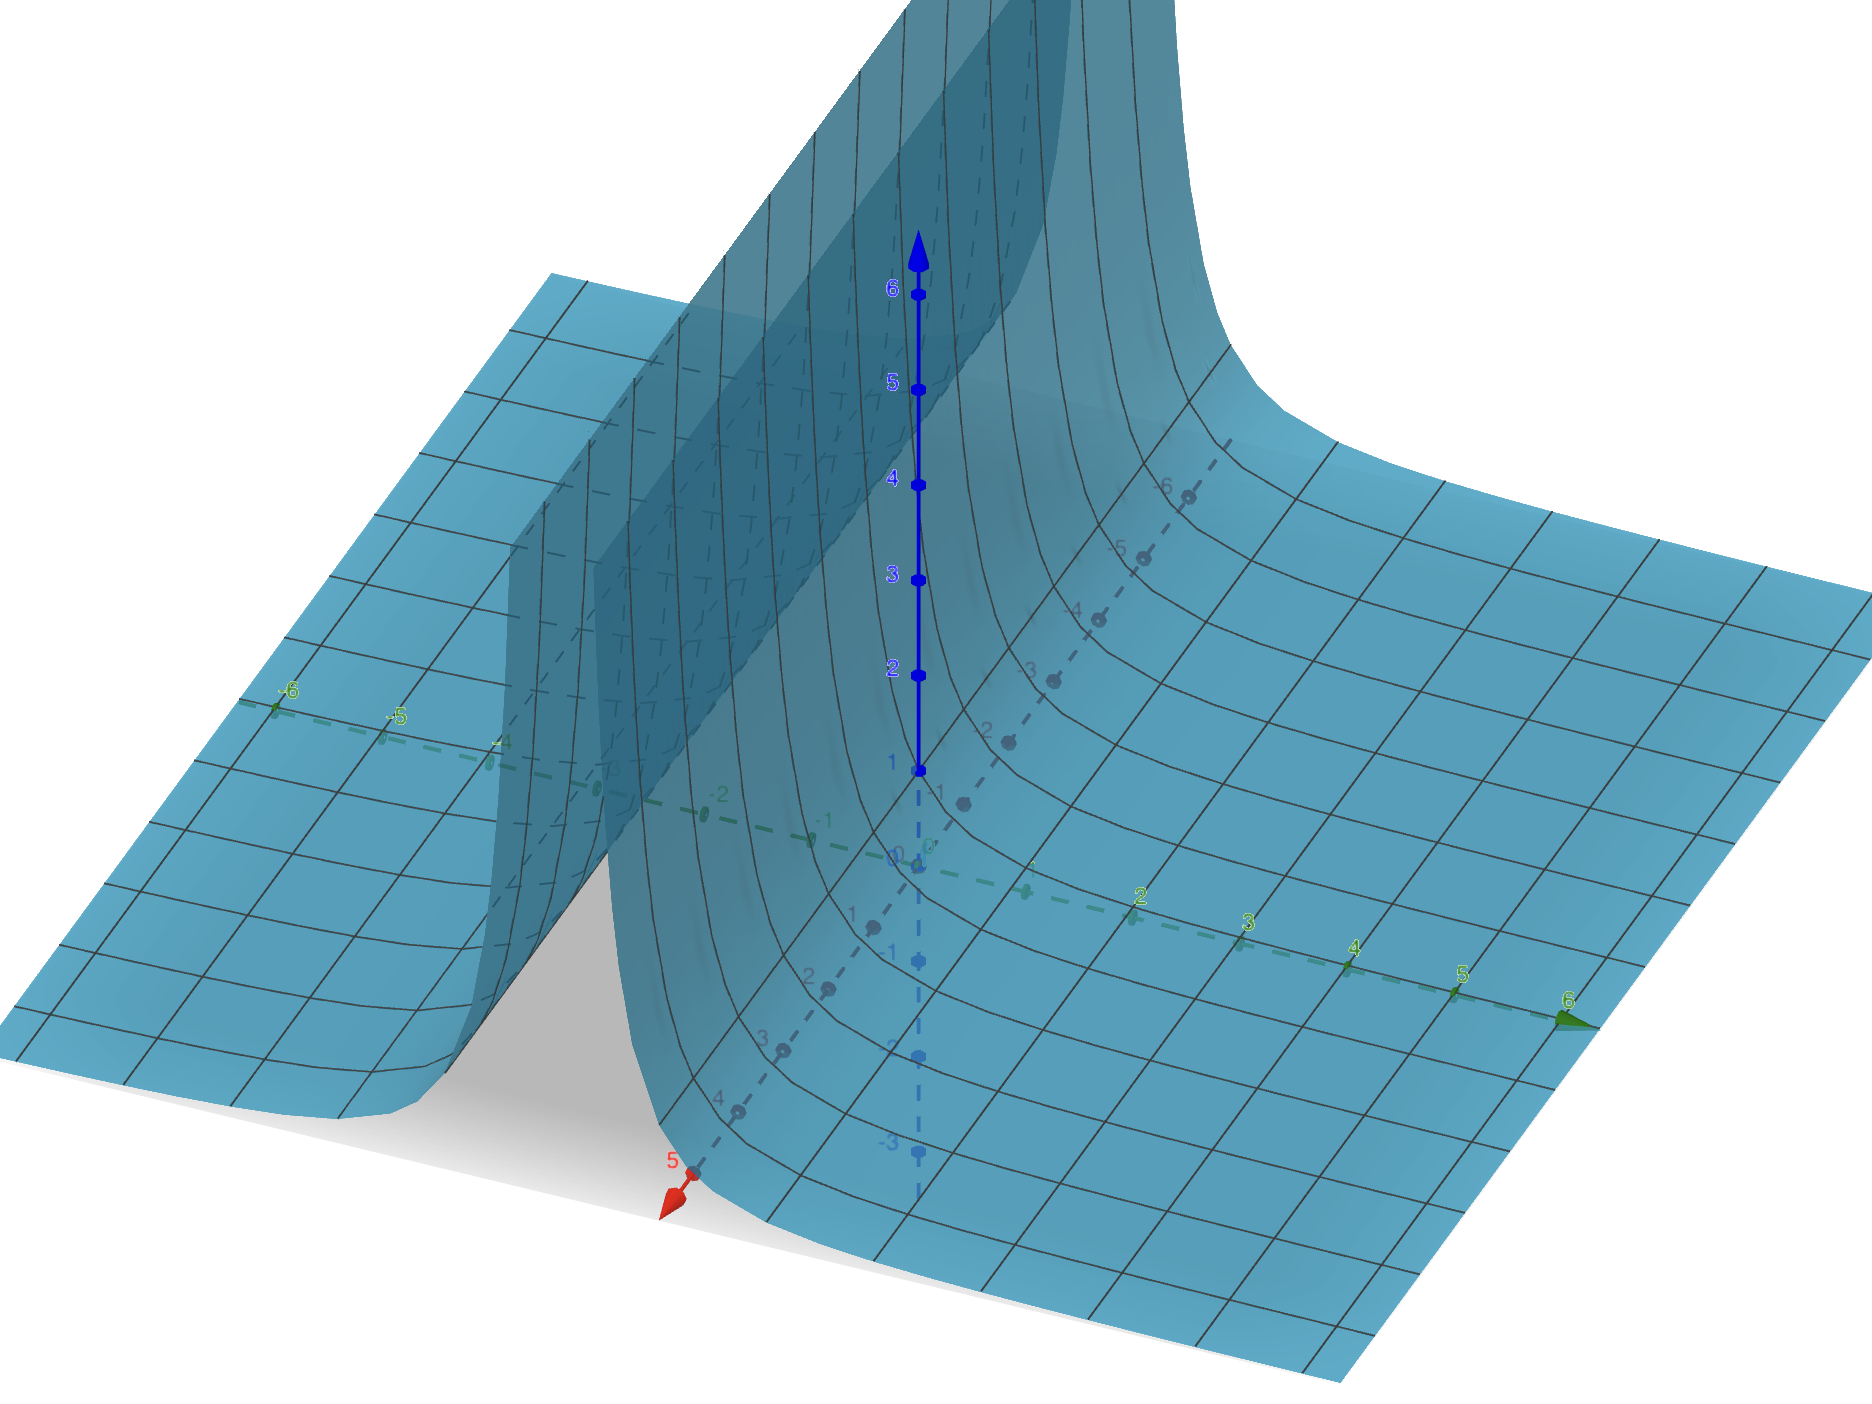
\includegraphics[scale=0.25]{images/Screenshot 2023-01-04 at 18.42.09.png}
        \caption{picture of $f(x,y)=\frac{1}{(y+1)^2}$}
    \end{figure}
    \begin{figure}[ht]
        \centering
        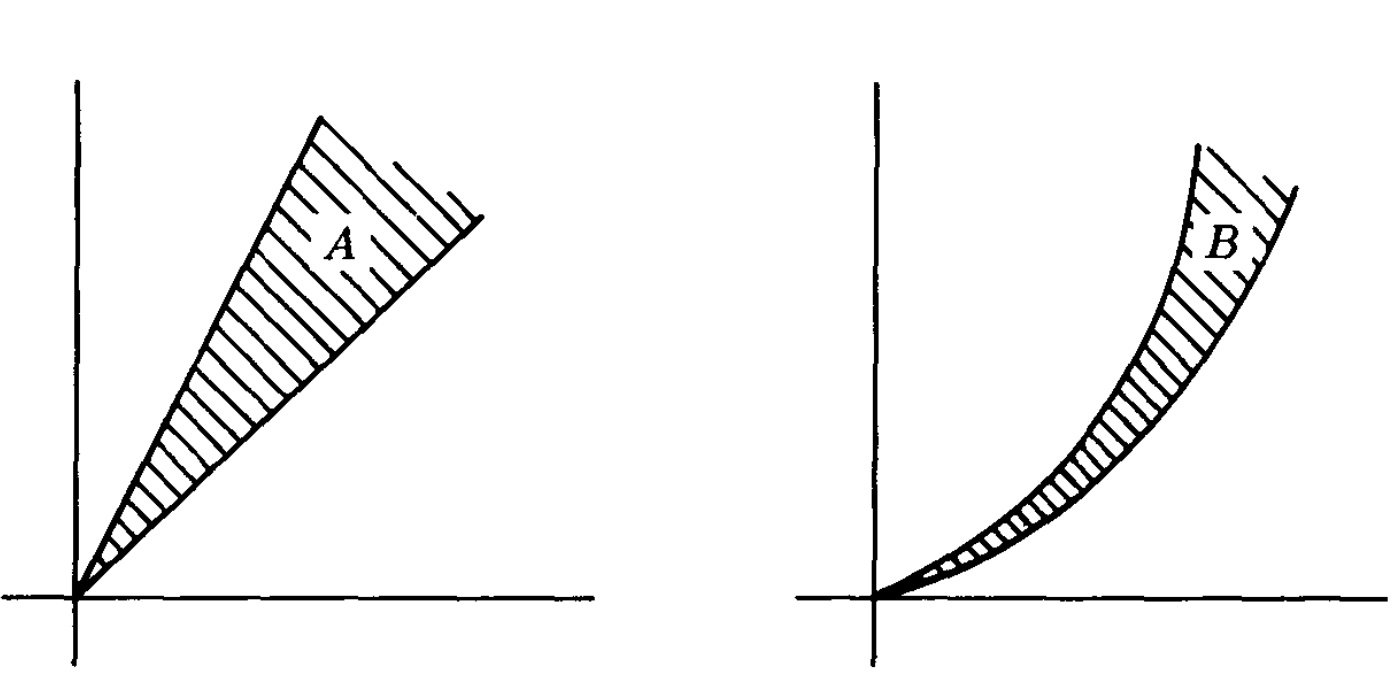
\includegraphics[scale=0.4]{images/Screenshot 2023-01-04 at 18.46.45.png}
        \caption{picture of $A,B$}
    \end{figure}
    \begin{enumerate}
        \item We show that $f$ is not integrable over $A$. Let $$U_N=\{(x,y):x\in(0,N)\text{ and }x< y< 2x\}$$
        With similar argument of the last example, we have 
        \begin{equation}
            \begin{split}
                \int_{U_N}|f| &= \int_{U_N}f\\
                &= \int_{\overline{U_N}}f\\
                &= \int_{x\in[0,N]}\int_{y=x}^{y=2x}\frac{1}{(y+1)^2}\di y\di x\\
                &= \int_{x\in[0,N]}(-\frac{1}{2x+1}+\frac{1}{x+1})\di x\\
                &= \log(N+1)
            \end{split}
        \end{equation}
        Taking the limit we have $$\lim_{N\to \infty}\log(N+1)=\infty$$
        So $f$ is not integrable over $A$.
        \item For the open set $B$, we set $$U_N=\{(x,y):x\in(0,N)\text{ and }x^2< y< 2x^2\}$$
        With similar argument of the last example, we have 
        \begin{equation}
            \begin{split}
                \int_{U_N}|f| &= \int_{U_N}f\\
                &= \int_{\overline{U_N}}f\\
                &= \int_{x\in[0,N]}\int_{y=x^2}^{y=2x^2}\frac{1}{(y+1)^2}\di y\di x\\
                &= \int_{x\in[0,N]}(-\frac{1}{2x^2+1}+\frac{1}{x^2+1})\di x\\
                &= \left(\arctan(x)-\frac{\arctan(\sqrt{2}x)}{\sqrt{2}}\right) \bigg\rvert_0^N\\
                &= \arctan(N)-\frac{\arctan(\sqrt{2}N)}{\sqrt{2}}
            \end{split}
        \end{equation}
        Taking the limit we have $$\lim_{N\to\infty}\arctan(N)-\frac{\arctan(\sqrt{2}N)}{\sqrt{2}}=\frac{\pi}{2}\left(1-\frac{1}{\sqrt{2}}\right)$$
        So $f$ is integrable over $B$.
        \begin{equation}
            \begin{split}
                \int_Bf &= \lim_{N\to\infty}\int_{U_N}f\\
                &= \lim_{N\to\infty}\arctan(N)-\frac{\arctan(\sqrt{2}N)}{\sqrt{2}}\\
                &=\frac{\pi}{2}\left(1-\frac{1}{\sqrt{2}}\right)
            \end{split}
        \end{equation}
    \end{enumerate}
\end{itemize}